\documentclass[a4paper,11pt]{article}

\usepackage[french]{babel}
\usepackage[a4paper,margin=2cm]{geometry}
\usepackage{hyperref}
\usepackage{listings}
\usepackage{xcolor}
\usepackage{fancyhdr}
\usepackage{amsmath,amssymb}
\usepackage{ulem}
\usepackage{emoji}
\usepackage{tikz}
\usepackage{tabularx}
\usepackage{pifont}
\usepackage{enumitem}



\lstset{
    basicstyle=\ttfamily\small,
    keywordstyle=\color{blue},
    commentstyle=\color{gray},
    stringstyle=\color{red},
    frame=single,
    numbers=left,
    numberstyle=\tiny\color{gray},
    breaklines=true,
    captionpos=b,
    language=[LaTeX]{TeX}
}

\hypersetup{
    colorlinks=true,
    linkcolor=blue,
    urlcolor=blue,
    pdfauthor={Votre Nom},
    pdftitle={Documentation du package A2SUP},
    pdfsubject={Package LaTeX},
    pdfkeywords={LaTeX, Package, Documentation}
}


\pagestyle{fancy}
\fancyhead[L]{\texttt{A2SUP}}
\fancyhead[R]{Documentation}
\fancyfoot[C]{\thepage}

\setlength{\parindent}{0pt}

\begin{document}

% Page de titre
\title{\textbf{Documentation du package \texttt{A2SUP}}}
\author{Abdussamed Yazici \\
\vspace{0.5em}
\small \texttt{samedyazici1905@gmail.com}}
\date{\today}

\maketitle

\medskip

\begin{center}
    \href{https://www.overleaf.com/read/dbchfhxfrhwx#c51201}{Package A2SUP -- A2Latex}
\end{center}

\begin{center}
    
\includegraphics[width=0.5\linewidth]{img/Turquie.png}
\end{center}



\tableofcontents
\newpage


\section{Introduction}
Le package \texttt{A2SUP} est conçu pour rédiger les supports de l'A2SUP, à destination des PASS et des L.AS. Il concerne les tutos, les GTs, les polycopiés d'exercices et de QCMs, les extras, et les packs de fiches (ces derniers étant utilisés pour les L.AS jusqu'à aujourd'hui).

Dans le passé, deux versions de \texttt{A2SUP.sty} existaient\footnote{Elles faisaient partie des projets "Archive PASS" et "Archive L.AS"}, pour chacune des voies d'accès. Désormais, les deux ont fusionné, et le seul et unique package \texttt{A2SUP.sty} se trouve dans le projet \href{https://www.overleaf.com/read/dbchfhxfrhwx#c51201}{\texttt{A2Latex}}.

Ce document détaille l'utilisation de \texttt{A2SUP.sty} en donnant des exemples pour chaque commande.





\section{Importation de \texttt{A2SUP.sty}}\label{Importation}
Pour pouvoir utiliser le package, il faut rendre disponible, dans le compte Overleaf d'intérêt, le projet \href{https://www.overleaf.com/read/dbchfhxfrhwx#c51201}{\texttt{A2Latex}}\footnote{\url{https://www.overleaf.com/read/dbchfhxfrhwx\#c51201}}.\\

Il n'y a qu'à cliquer sur le lien, et rejoindre le projet avec un compte Overleaf.\\

Maintenant que le projet est disponible, il est possible d'ouvrir un projet Overleaf (pour un tuto par exemple), puis d'\textbf{importer directement} depuis le projet \texttt{A2Latex} les fichiers \texttt{A2SUP.sty} et \texttt{logo.png}.\\

Voici un tutoriel vidéo si besoin : \url{https://shorturl.at/4nUIz}


% Utilisation de base
\section{Commandes de \texttt{A2SUP.sty}}

Dans cette section, nous allons expliquer les commandes du package, en les sélectionnant dans l'ordre d'apparition dans un document (voir section \ref{template}).

\subsection{\texttt{\textbackslash documentclass[12pt]\{article\}}}

C'est la première ligne obligatoire de tout document. Elle permet de déclarer que le document est un article, rédigé en taille de police 12pt. Ne pas oublier donc de bien indiquer que la taille est de 12pt !

\subsection{\texttt{\textbackslash usepackage\{A2SUP\}}}

Cette ligne permet d'importer l'ensemble des codes se trouvant dans \texttt{A2SUP.sty}. Il est donc nécessaire que le fichier \texttt{A2SUP.sty} soit présent dans le projet. Se rendre à la section \ref{Importation} si besoin.\\

Ce package ne peut être utilisé qu'avec le compilateur Lua\LaTeX{}. Par défaut, les projets Overleaf et PLMLatex sont configurés avec le compilateur pdfLaTeX. Il faudra donc changer le compilateur pour un projet nouveau : \url{https://shorturl.at/KPItf}\\


\verb|\usepackage{A2SUP}| présente des options :

\begin{itemize}
    \item \verb|\usepackage[année=2020-2021]{A2SUP}|\\
        Par défaut, le package est configuré sur l'année en cours. Mais il est possible de changer l'année d'un support (utile pour les annales par exemple). \textbf{Attention}, \verb|année|, et non \verb|annee| !
    \item \verb|\usepackage[correction=blue!1!white]{A2SUP}|\\
        Les blocs de correction, codés par l'environnement \texttt{correction} (\ref{correction}), ont un fond coloré (par défaut fixé sur \texttt{red!1!white}). Il est donc possible de modifier la couleur. Ici, toutes les boites de correction seront colorées en \texttt{blue!1!white}\footnote{\textsl{À noter que \texttt{blue!1!white} renvoie une couleur issue d'un mélange de $1\%$ de bleu et $100-1=99\%$ de blanc}}. Mais il est possible de ne modifier la couleur que d'une seule boite de correction (\ref{correction}).
    \item \verb|\usepackage[boite=yellow!1!white]{A2SUP}|\\
        De la même manière que l'environnement \texttt{correction}, l'environnement \texttt{boite} (\ref{boite}) donne une petite boite colorée, dont la couleur par défaut est \texttt{blue!1!white}. Ici, toutes les boites qui seront générées dans le document seront de couleur \texttt{yellow!1!white}, mais il est aussi possible de déterminer la couleur d'une boite en particulier (voir \ref{boite}).
    \item \verb|\usepackage[plan=oui]{A2SUP}|\\
        Par défaut, \texttt{plan=non}. Quand il est égal à oui, la MEP des titres, sous-titres et sous-sous-titres est modifiée. Les titres (\verb|\section{...}|) sont alors rouges, les sous-titres (\verb|\subsection{...}|) bleues, et les sous-sous-titres (\verb|\subsubsection{...}|) vertes. Si non, tout est noir, et la taille de police est légèrement plus faible.
\end{itemize}

\bigskip

Les options sont cumulables, séparées par une virgule. Il est donc possible de poser :

\begin{lstlisting}
\usepackage[plan=oui, boite=pink!1!white, année=2019-2020]{A2SUP}
\end{lstlisting}


\subsection{Environnement \texttt{informations}}\label{informations}

Cet environnement permet de donner toutes les informations concernant le support. Tout l'intérêt de l'utilisation de \LaTeX{} pour nos supports réside dans cet environnement : sans toucher au contenu du projet, on est capable de générer un tuto plutôt qu'un GT ; plus besoin de supprimer toutes les corrections pour obtenir le sujet ; pas de perte de temps avec la pagination...\\

Cet environnement, comme tout environnement, est structuré de cette façon :

\begin{lstlisting}
\begin{informations}
    <contenu>
\end{informations}
\end{lstlisting}

En l'occurrence, voici le contenu :


\begin{lstlisting}
\begin{informations}
    UE = ,
    Support = ,
    NumeroDuSupport = ,
    SujetOuCorrection = ,
    Orientation = ,
    Pagination = ,
    TiersTemps = ,
    RecoSpecifiques = ,
    TitreExtra = ,
    SousTitre = ,
    Redacteurs = ,
    Relecteurs = ,
    ConvertisseursLatex = ,
    Testeurs = ,
    TuteursEnSeance = ,
    VP = ,
    Team = ,
    RM = ,
    FacRedactionOuCollab = ,
    RemerciementsBonus = ,
    Session = ,
    RelectureProfs = ,
\end{informations}
\end{lstlisting}

\newpage

Les éléments ici sont des \textbf{clés}. Chaque clé peut prendre une valeur, créant alors un couple clé-valeur :

\begin{itemize}
    \item \texttt{UE = ...}\\
        Pour les PASS $\rightarrow$ \uline{1 à 11}. Pour les UE12 : \uline{12med}, \uline{12odonto}, \uline{12maieu}, \uline{12pharma}\\
        Pour les L.AS $\rightarrow$ \uline{1.1} ou \uline{1.2} ou \uline{2.1} ou \uline{2.2} ou \uline{3.1} ou \uline{3.2} ou \uline{4.1} ou \uline{4.2}
    \item \texttt{Support = ...}\\
        \uline{tuto}, \uline{GT}, \uline{poly d'exos}, \uline{poly de QCM}, \uline{annale}, \uline{extra}, \uline{fiche} (et \uline{pack} uniquement pour les L.AS)
    \item \texttt{NumeroDuSupport = ...}\\
        Indiquer tout simplement le numéro (2 pour un tuto 2 par exemple)
    \item \texttt{SujetOuCorrection = ...}\\
        \uline{sujet} ou \uline{correction}, en sachant que par défaut, le support est en version sujet (possible de ne pas donner de valeur si l'on veut un sujet, ou un support comme une fiche)
    \item \texttt{Orientation = ...}\\
        \uline{paysage} ou \uline{portrait}. La valeur par défaut dépend de la valeur de \texttt{SujetOuCorrection} (portrait si sujet, paysage si correction). Il est possible de demander une correction en portrait, ou un sujet en paysage !
    \item \texttt{Pagination = ...}\\
        \uline{oui} ou \uline{non} (valeur par défaut : oui). À noter que la pagination se fait en fonction de l'orientation du support : en bas au centre si document en paysage ; en bas à droite si document en portrait.
    \item \texttt{TiersTemps = ...}\\
        \uline{oui} ou \uline{non} (valeur par défaut : non). Permet d'augmenter l'interligne (1.5), et la taille de police (14pt).
    \item \texttt{RecoSpecifiques = ...}\\
        La valeur constituera les recommandations spécifiques affichées sur la page de couverture des tutos. Veiller à mettre des accolades si la valeur contient une ou des virgule(s) (cf remarque faite après la liste pour plus de détail).
    \item \texttt{TitreExtra = ...}\\
        La valeur s'affichera sur la page de couverture d'un extra (elle prend généralement le type du support, comme "Tableau comparatif", ou "Rappels"... Libre à vous...). Veiller à mettre des accolades si la valeur contient une ou des virgule(s) (cf remarque faite après la liste).
    \item \texttt{SousTitre = ...}\\
        La valeur s'affichera en sous-titre sur la page de couverture d'un extra (généralement le nom du ou des cours) ou d'une fiche (généralement le nom du cours). Pour un extra, \texttt{SousTitre} est accompagné de \texttt{TitreExtra}. Pour une fiche, \texttt{SousTitre} est accompagné de "Fiche \texttt{NumeroDuSupport}". Veiller à mettre des accolades si la valeur contient une ou des virgule(s) (cf remarque faite après la liste).
    \item \texttt{Redacteurs = {...}}\\
        Prenom NOM (Filière, Poste CA si existe), ... Remarquer qu'il y a TRÈS souvent des virgules dans la valeur assignée, puisqu'il y a plusieurs rédacteurs. Il ne faut donc surtout pas oublier les accolades !
    \item \texttt{Relecteurs = {...}}\\
        Prenom NOM (Filière, Poste CA si existe), ... Remarquer qu'il y a TRÈS souvent des virgules dans la valeur assignée, puisqu'il y a plusieurs relecteurs. Il ne faut donc surtout pas oublier les accolades ! Si valeur vide, rien ne s'affiche dans la page de remerciements.
    \item \texttt{ConvertisseursLatex = {...}}\\
        Prenom NOM (Filière, Poste CA si existe), ... Remarquer qu'il peut y avoir des virgules dans la valeur assignée, puisqu'il peut y avoir plusieurs convertisseurs \LaTeX{}. Il ne faut donc surtout pas oublier les accolades ! Si valeur vide, rien ne s'affiche dans la page de remerciements.
    \item \texttt{Testeurs = {...}}\\
        Prenom NOM (Filière, Poste CA si existe), ... Concerne des personnes qui auraient tester un tuto classiquement (mais pourquoi pas un GT ou autre...). Ne pas oublier les accolades si la valeur contient une ou des virgules. Si valeur vide, rien ne s'affiche dans la page de remerciements.
    \item \texttt{TuteursEnSeance = ...}\\
        Prenom NOM (Filière, Poste CA si existe), ... Concerne des personnes qui ont donné des séances de GT ou de souk. Ne pas oublier les accolades si besoin. Si valeur vide, rien ne s'affiche dans la page de remerciements.
    \item \texttt{VP = ...}\\
        Prenom NOM (Filière), ... Indiquer les VP Tuto actuels. Ne pas oublier les accolades si besoin.
    \item \texttt{RM = ...}\\
        Prenom NOM (Filière, Poste CA si besoin), ... Indiquer les RM impliqués. Ne pas oublier les accolades si besoin.
    \item \texttt{FacRedactionOuCollab = ...}\\
        \uline{rédaction} ou \uline{collaboration} (valeur par défaut : collaboration). Permet d'afficher l'implication de la fac dans la page de remerciements. La fac est supposée au moins collaboratrice, automatiquement (cf valeur par défaut).
    \item \texttt{RemerciementsBonus = ...}\\
        Exploiter cette clé si besoin de faire des remerciements occasionnels (les RM de maths ont pu remercier le studio qui leur avait permis de tourner leurs vidéos par exemple). Si valeur vide, rien ne s'affiche dans la page de remerciements.
    \item \texttt{Session = ...}\\
        Spécifique aux annales. Sa valeur s'affiche dans la page de couverture du support, pour indiquer de quelle session il s'agit (2020-2021 Tuto 1, ou 2020-2021 Session 1).
    \item \texttt{RelectureProfs = ...}\\
        "oui", ou "non" ("non" par défaut). Cette clé permet, pour une correction, de ne pas afficher les blocs de correction. Il est ainsi simple d'obtenir une correction ne contenant que des questions ainsi que leur bilan de réponse, sans correction détaillée, que les professeurs pourront relire.
\end{itemize}

\bigskip

\emoji{warning} Pour toute valeur contenant une ou plusieurs virgules, il est \textbf{nécessaire} de mettre la valeur entre accolades \{\}, car les virgules sont utilisées pour séparer les couples clé-valeur !! Ainsi :\\

\verb|TitreExtra = {Os, et cartilage},| et non \verb|TitreExtra = Os, et cartilage,|\\

Pour un support donné, si la clé n'est pas utilisée, alors elle peut être vide. Par exemple, inutile d'indiquer quoique ce soit pour \verb|TitreExtra| si le support est un tuto !



\subsection{Environnement \texttt{document}}

Cet environnement pose les limites du document PDF. Tout ce qui se trouve avant l'environnement est dans le \textbf{préambule}. Tout ce qui se trouve après l'environnement n'est pas traité par \LaTeX{}, il est complètement ignoré.

\begin{lstlisting}
<préambule>

\begin{document}
    <contenu donnant le PDF>
\end{document}
\end{lstlisting}


\subsection{\texttt{\textbackslash recto}}

\verb|\recto| donne simplement la page de couverture là où est placée la commande. À savoir que la commande s'occupe déjà du fait que la page de couverture occupe une page entière, et que le contenu suivant se situe sur la page suivante. Inutile de demander un saut de page donc ! La page de couverture se met en page en fonction de la valeur de la clé \verb|Support| de l'environnement \verb|informations|.\\

Pour les tutos et annales, le nombre de pages, ainsi que le nombre de questions dans le document sont calculés automatiquement. Nul besoin de préciser ces informations. Il en est de même pour l'autorisation de l'utilisation d'une calculatrice. Si vous remarquez que l'autorisation n'est pas conforme, faites la demande et le projet \texttt{A2Latex} sera réactualisé.\\

Pour les packs de fiches, et uniquement pour les packs de fiches, la commande \verb|\recto| prend un argument optionnel : \verb|\recto[]|. L'argument contiendra les fiches que le pack compile.

\begin{lstlisting}
\recto[
    -- Fiche n°1\\
    -- Fiche n°2
]
\end{lstlisting}

Voici un exemple de projet si vous voulez voir comment est géré un pack de fiches : \href{https://www.overleaf.com/read/jmnjqkqxpmnm\#736a88}{Pack de fiches n°1 de Biophysique L.AS}\footnote{\url{https://www.overleaf.com/read/jmnjqkqxpmnm\#736a88}}

\subsection{\texttt{\textbackslash grille}}

Cette commande ajoute la grille là où se trouve la commande. À savoir que la grille ne s'affiche que dans la correction du support, et qu'il est possible d'obtenir une grille vierge en appelant \verb|\grille[vierge]|.\\

Le remplissage automatique de la grille est réalisé à l'aide des bilans de réponse donnés au fur et à mesure de la correction. \textsl{Pour les plus curieux, \LaTeX{} fait cela en créant un fichier auxiliaire \texttt{bilans.aux}}.

\subsection{Environnement \texttt{motRM}}

Cet environnement permet d'ajouter le mot du RM, selon ce format :

\begin{lstlisting}
\begin{motRM}[titre=Coucou les P1 !, couleur=red!1!white, afficher=toujours]
    <contenu>
\end{motRM}
\end{lstlisting}

L'environnement n'isole pas automatiquement le mot des RM dans une page. Si vous voulez que les éléments suivants le mot des RM se trouvent sur la page suivante, il est nécessaire de demander un saut de page, via \verb|\newpage|. L'environnement est codé comme cela pour permettre de positionner plusieurs mots de RM sur une même page, par exemple.\\

Options de l'environnement \verb|motRM| :

\begin{itemize}
    \item \texttt{titre=...}\\
        Prend pour valeur le titre du mot. Il est automatiquement mis en gras, souligné et de taille de police légèrement agrandie. \textbf{Ne pas oublier de mettre la valeur entre accolades si elle contient une ou des virgules !}
    \item \texttt{couleur=...}\\
        Pour spécifier une couleur si souhaité, en sachant qu'il y a une couleur par défaut, et qu'il n'est donc pas nécessaire d'appeler l'option.
    \item \texttt{afficher=...}\\
        \uline{sujet}, \uline{correction} ou \uline{toujours}. Assez explicite. Par défaut, le mot des RM ne s'affiche que dans la correction. Inutile d'appeler cette option si vous ne le voulez que dans la correction donc.
\end{itemize}


\bigskip

Voici le minimum nécessaire :

\begin{lstlisting}
\begin{motRM}[titre={Coucou, les P1 !}]
    <contenu>
\end{motRM}
\end{lstlisting}

Notez les accolades, protégeant la virgule de la valeur de titre \emoji{wink}.


\subsection{\texttt{\textbackslash question}}

Cette commande, contenant 8 arguments obligatoires, permet de mettre en page la question ainsi que ses items, tout en recensant le bilan de réponse. La mise en page de la question sera dépendante de l'UE indiquée (pour la suite, on prendra l'UE9). Si la MEP utilisée n'est pas conforme à l'UE, contacter Abdussamed pour les modifications.

\begin{center}
    \begin{tikzpicture}
        \draw[fill=blue!3!white] (0.1, -0.2) rectangle (2.1, 0.25);
        \node at (0,0) {\texttt{\textbackslash question\{\}\{\}\{\}\{\}\{\}\{\}\{\}\{\}}};
        \draw[latex-, color=blue!40!black] (-0.55,-0.2) to [looseness=1, out=-110, in=80] (-2.5,-0.8) node[below] {n°};
        \draw[latex-, color=blue!40!black] (-0.15,-0.2) to [looseness=1, out=-110, in=70] (-2.25,-1.8) node[below] {Énoncé};
        \draw[latex-, color=blue!40!black] (1.15,-0.2) to [looseness=1, out=-70, in=110] (2.2,-1.75) node[below] {Items A à E};
        \draw[latex-, color=blue!40!black] (2.3,-0.2) to [looseness=1, out=-70, in=110] (4,-1) node[below] {bilan};
    \end{tikzpicture}
\end{center}

\uline{Conseil} :\\
Préférer la mise en page suivante pourrait grandement faciliter la relecture et la lisibilité des fichiers (essayer donc au maximum de l'appliquer) \textsl{(cependant, attention à ne pas séparer des paires d'accolades par une ligne vide !)}.

\begin{lstlisting}
\question{1}
{Enoncé}
{Item A}
{Item B}
{Item C}
{Item D}
{Item E}
{AE}
\end{lstlisting}

\subsubsection{Numéro de la question}

Indiquer simplement le numéro de la question avec des chiffres arabes, et uniquement avec des chiffres arabes, au risque d'induire des erreurs au niveau de la grille de correction. 


\subsubsection{Énoncé}

Il est possible d'écrire des énoncés longs et s'étendant sur plusieurs paragraphes. Il est possible d'ajouter des tableaux, des images, et autres types de contenu, à vous de trouver de l'originalité ! Faites seulement attention à BIEN garder les deux accolades !

\begin{lstlisting}
\question{1}
{
    Un système astrophysique est constitué d'un disque d'accrétion en rotation
    autour d'un trou noir supermassif. Ce disque est composé de plasma chaud, 
    fortement ionisé, et soumis à un champ magnétique complexe qui s'étend dans 
    l'espace environnant.\\

    Des observations récentes montrent des jets relativistes de matière éjectés
    perpendiculairement au plan du disque, atteignant des vitesses proches de 
    la vitesse de la lumière. Ces jets transportent de grandes quantités 
    d'énergie et présentent des structures de polarisation magnétique qui
    changent dynamiquement avec le temps.

    \begin{center}
        \includegraphics[width=0.3\linewidth]{example-image-duck}
    \end{center}
}
{La mer noire}
{Poudre de perlimpinpin}
{Oui (fi)}
{Quoi (feur)}
{Trivial}
{ABE}
\end{lstlisting}

Voici le rendu :

\begin{center}
    \fcolorbox{red!30}{red!30}{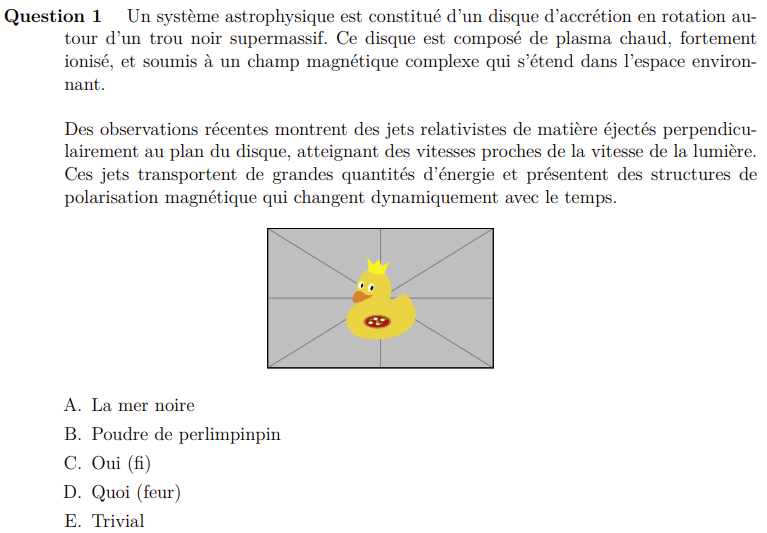
\includegraphics[width=0.5\linewidth]{img/énoncé.png}}
\end{center}

Essayer de garder cette mise en page, qui est très agréable, espacée, et qui permet de se retrouver rapidement. Pour déplacer un ensemble de paragraphes, sélectionner les paragraphes (en glissant la souris dessus), et taper \verb|Tab|. Inutile de sélectionner rigoureusement les paragraphes, il est suffisant de sélectionner une partie d'un paragraphe pour qu'il soit en retrait de la marge. Voici un tutoriel vidéo pour illustrer : \url{https://shorturl.at/rglTy}\\

A noter :

\begin{itemize}
    \item Un retour à la ligne se fait en laissant une ligne vide entre une phrase $n$ et une phrase $n+1$ que vous souhaitez placer en retour de ligne.
    \item Un saut de ligne entre deux paragraphes se fait à l'aide de \verb|\\|, suivi d'une ligne vide.
    \item Avant et après TOUT environnement, il n'est pas correct de mettre \verb|\\|. C'est la raison pour laquelle je n'en mets pas avant l'environnement \verb|center|, qui prend déjà en compte un espacement vertical \textbf{avant}, et \textbf{après}. Si l'espacement vertical ne vous plaît pas (à éviter en général...), vous pouvez jouer sur cet espacement avec les commandes \verb|\smallskip|, \verb|\medskip| et \verb|\bigskip|, en sachant qu'elles sont cumulables (mettre deux fois \verb|\smallskip| revient à sommer les deux espaces).
    \item Une image se place à l'aide de la commande :
    
        \begin{center}
            \verb|\includegraphics[width=...\linewidth]{nom_de_l'image}|
        \end{center}
        
        Ici, on définit la largeur de l'image, de façon relative à la largeur de la feuille (plus juste, quand on sait qu'on travaille sur des supports parfois portrait, parfois paysage). A savoir qu'il est aussi possible de définir non pas la largeur, mais la hauteur via \verb|height=...\pageheight| (mêmes remarques avec la hauteur de la page cette fois). A noter enfin qu'il est quand même possible de placer des longueurs en \verb|cm|, ou \verb|mm| (mais les longueurs relatives restes plus souhaitables). Évidemment, il est nécessaire que l'image soit présent dans le projet. Voici une astuce rapide pour ajouter une image sur Overleaf : \url{https://shorturl.at/gKPgc}
\end{itemize}





\bigskip


Étant donné que j'ai parlé de la possibilité d'ajouter un tableau, j'en profite pour montrer un code contenant un tableau simple :


\begin{lstlisting}
\question{1}
{
    Voici le tableau suivant :

    \begin{center}
        \begin{tabular}{|c|l|r|}
            \hline
                        & \textbf{Col 1} & \textbf{Col 2} \\
            \hline
                ligne 1 & Waw            & Waw \\
            \hline      
        \end{tabular}
    \end{center}

    Que pensez-vous de ce tableau ?
}
{Euh...}
{Heja le top}
{Mouais fin bon, de toute façon, il n'y aura plus d'eau dans 5 ans si mes
calculs sont bons...}
{Qui s'en tape ? \emoji{hand}}
{Trivialement trivial}
{BDE}
\end{lstlisting}




Voici le rendu :


\begin{center}
    \fcolorbox{red!30}{red!30}{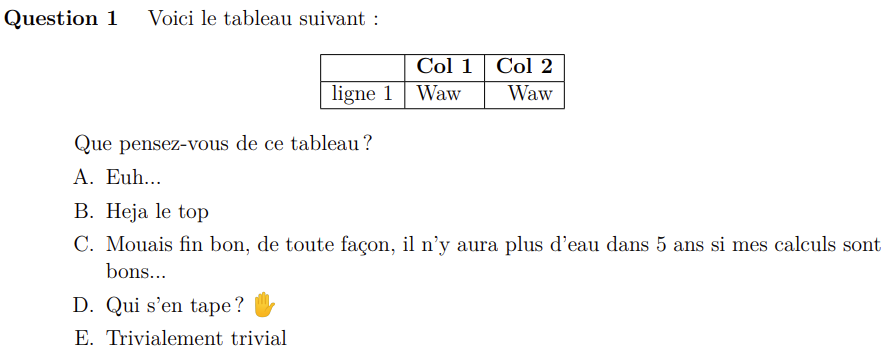
\includegraphics[width=0.7\linewidth]{img/question_avec_tableau.png}}
\end{center}


Pour plus d'informations sur les tableaux, rendez-vous à la section \ref{tableaux}.












\subsubsection{Aide aux calculs}\label{aide_au_calcul}

Si la question comporte des aides aux calculs, elles doivent être indiquées dans l'argument contenant l'énoncé, comme ceci :

\begin{lstlisting}
\question{1}
{
    Enoncé\\
    
    Aide aux calculs : $\int_\mathbb R e^{-x^2}\, dx = \pi$ ; $1+1=11$ ; $9.99\approx 10$
}
{Item A}
{Item B}
{Item C}
{Item D}
{Item E}
{AE}
\end{lstlisting}










\subsubsection{Items}\label{Items}

Il n'y a qu'à indiquer le contenu de chaque item, sans nécessité de préciser de quel item il s'agit. Inutile donc de formuler l'item "A. Item A", "Item A" suffit. Évidemment, pas de point en fin d'item, donc "Item A", et non "Item A.". Le mode mathématique est possible en utilisant les \verb|$$|. Il est aussi possible d'ajouter une image si besoin.

\begin{lstlisting}
\question{1}
{Parmi les propositions suivantes, lesquelles sont exactes ?}
{Le calcul $1+1=2$ est vrai}
{
    \includegraphics[width=0.3\linewidth]{example-image-duck}
}
{$\ce{H3O+ + HO- <=> 2H2O}$}
{Ceci est l'item E}
{Vive \LaTeX{}}
{ABCE}
\end{lstlisting}

\begin{center}
    \fcolorbox{red!30}{red!30}{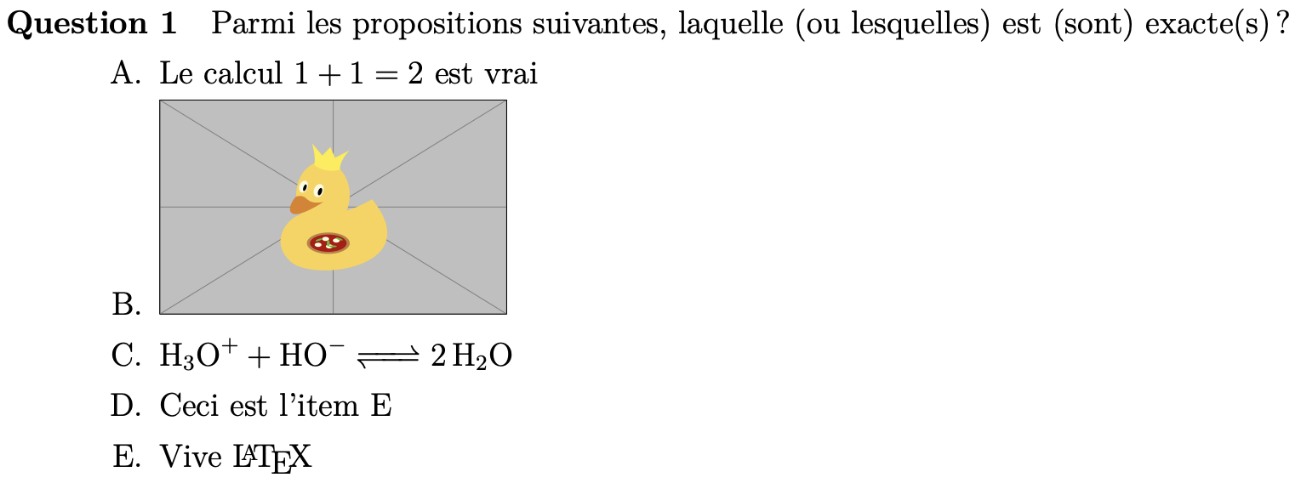
\includegraphics[width=0.7\linewidth]{img/Items.png}}
\end{center}


La commande \verb|\ce{}| vient du package \verb|mhchem| : \url{https://mirror.ibcp.fr/pub/CTAN/macros/latex/contrib/mhchem/mhchem.pdf}\\

À noter qu'il est impossible qu'un saut de page sépare les items et l'énoncé. Le tout forme un groupe solidaire. Attention donc à ne pas mettre d'image excessivement grande dans l'énoncé par exemple, pouvant mener à un débordement des items en bas de page (puisque \LaTeX{} forcera le positionnement d'un contenu de plus d'une page... sur \textbf{une} page).


\subsubsection{Bilan de réponse}

Le bilan de réponse contient uniquement les items vrais, les lettres étant en majuscule, sans virgule ni conjonction. Les bilans sont donc \verb|{ABE}|, \verb|{BC}| etc. Les items vrais doivent être donnés dans l'ordre alphabétique : \verb|{ABE}| et non \verb|{AEB}|. Pas de lettres intrus : \verb|{ABE}| et non \verb|{A, B et E}|.\\

Les bilans de réponse n'impactent pas la mise en page dans les sujets. Ce n'est que dans la correction qu'ils guideront la MEP des items corrigés. En reprenant le même code que dans la section \ref{Items} :

\medskip

\begin{minipage}{0.49\linewidth}
    \centering
    Dans le sujet :

    \medskip
    
    \fcolorbox{red!30}{red!30}{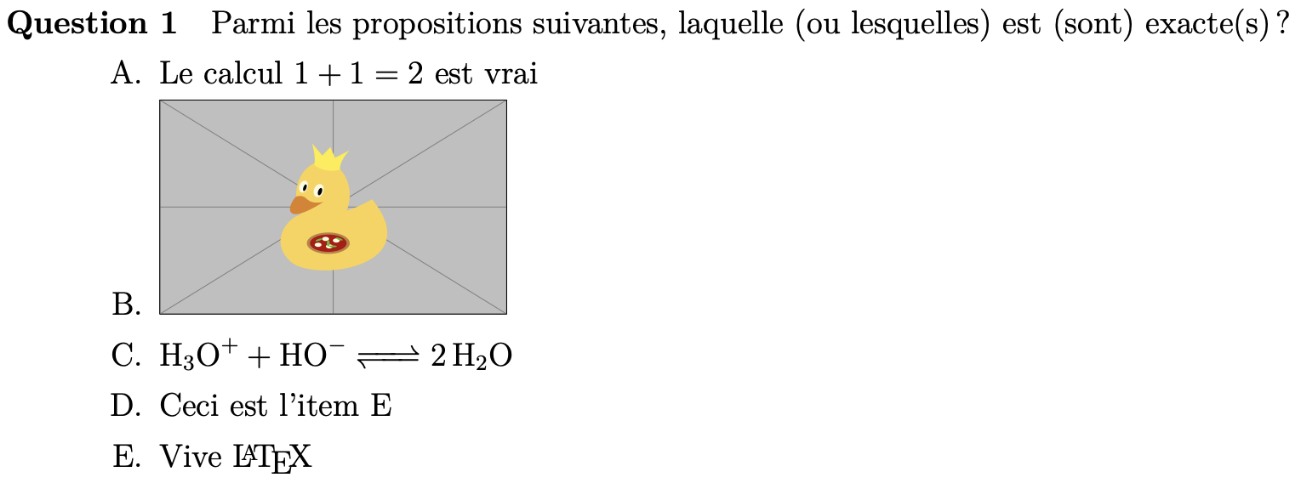
\includegraphics[width=\linewidth]{img/Items.png}}
\end{minipage}
\hfill
\begin{minipage}{0.49\linewidth}
    \centering
    Dans la correction :

    \medskip
    
    \fcolorbox{red!30}{red!30}{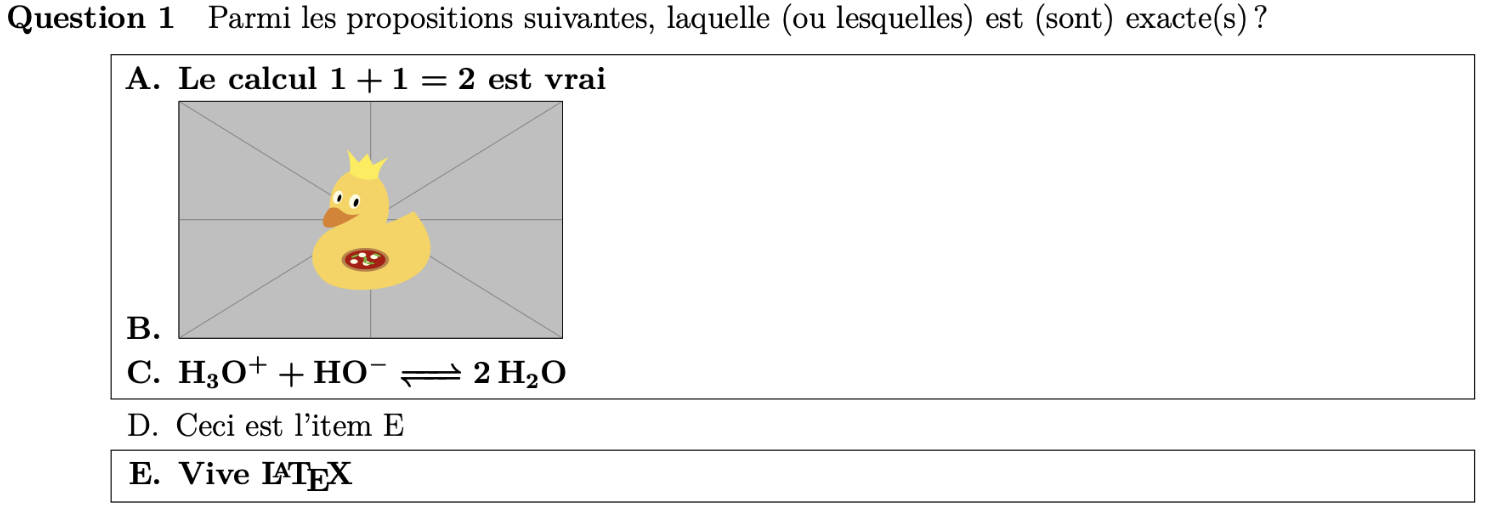
\includegraphics[width=\linewidth]{img/bilans.png}}
\end{minipage}

\medskip

De plus, en fonction du bilan de réponse donné, la correction qui arrive par la suite contiendra automatiquement un résumé ("Réponses vraies : A et E" si le bilan est \verb|{AE}| par exemple).\\

À noter qu'il est possible de ne rien indiquer dans le bilan de réponse (en laissant donc une paire d'accolades \verb|{}| vide). Dans ce cas, tous les items seront considérés faux. C'est un cas qui est arrivé dans une annale, suite à une erreur de la part des profs.

\subsubsection{Question hors programme}

Si vous souhaitez indiquer qu'une question entière est hors programme, il suffit d'utiliser la version étoilée \verb|\question*|, avec ses arguments habituels :

\begin{lstlisting}
\question*{1}
{Parmi les propositions suivantes, lesquelles sont exactes ?}
{Le calcul $1+1=2$ est vrai}
{
    \includegraphics[width=0.3\linewidth]{example-image-duck}
}
{$\ce{H3O+ + HO- <=> 2H2O}$}
{Ceci est l'item E}
{Vive \LaTeX{}}
{ABCE}
\end{lstlisting}

\begin{center}
    \fcolorbox{red!30}{red!30}{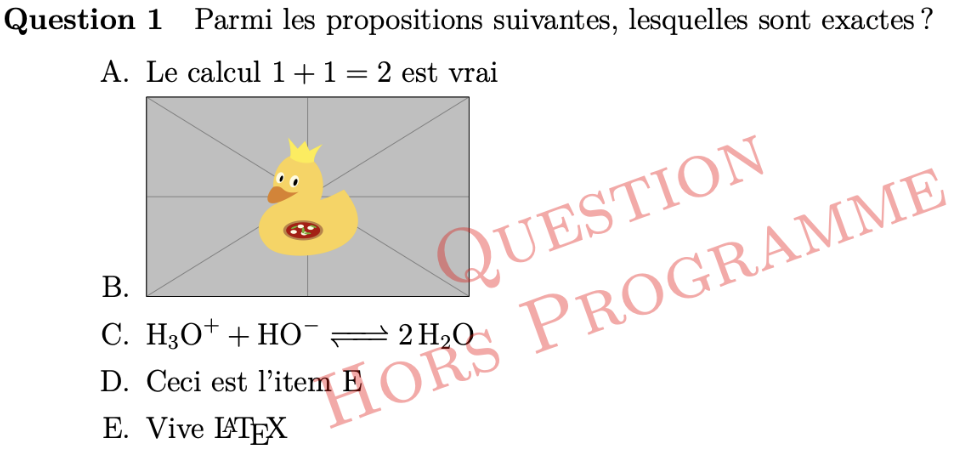
\includegraphics[width=0.7\linewidth]{img/question-HP.png}}
\end{center}

Je note par précaution que l'indication "Question hors programme" est bien centrée horizontalement. Ça n'a pas l'air ici à cause de l'extrait qui n'occupe pas toute la largeur de la page.





\subsection{\texttt{\textbackslash questionouverte}}

Cette commande fonctionne grossièrement de la même façon que \verb|\question|, à la différence que \verb|\questionouverte| ne contient que 2 arguments obligatoires (pour le numéro et l'énoncé de la question), et contient 7 arguments optionnels (pour 7 éventuelles questions). Il n'y a pas de possibilité d'indiquer des aides au calcul de façon intégrée comme avec la commande \verb|\question|, et il n'y a pas de bilan de réponse à indiquer. Néanmoins, \verb|\questionouverte| informe quand même \verb|\grille| sur le fait que la question étudiée est une question ouverte, et qu'il n'y a donc pas de réponse vraie, la grille pouvant alors "sauter" la question lors du remplissage des cases.

\begin{lstlisting}
\questionouverte{1}
{Répondez à l'ensemble de ces questions :}
[Qu'est-ce que la réalité, et comment pouvons-nous être sûrs qu'elle existe en 
dehors de notre perception ?]
[Sommes-nous libres de nos choix, ou tout est-il prédéterminé ?]
[Un acte est-il bon parce que Dieu le commande, ou Dieu le commande-t-il parce 
qu'il est bon ?]
[La solitude est-elle essentielle pour comprendre qui nous sommes ?]
[Quelle est la limite entre foi et raison ?]
[Peut-on connaître réellement les pensées ou émotions des autres ?]
\end{lstlisting}

\begin{center}
    \fcolorbox{red!30}{red!30}{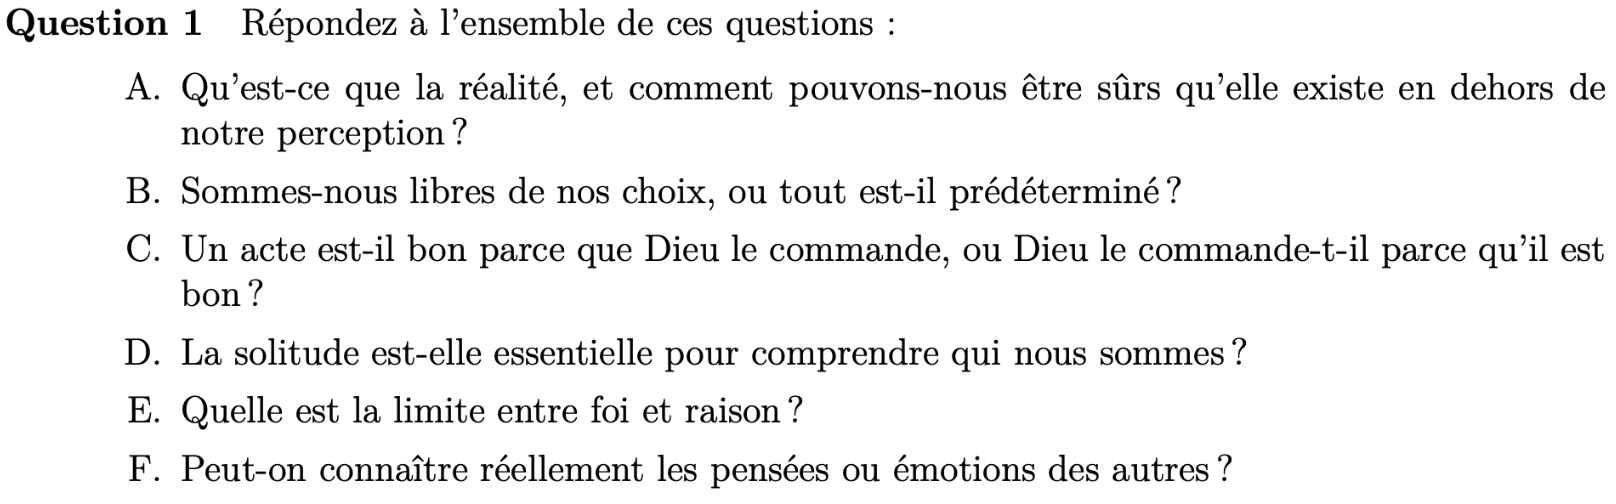
\includegraphics[width=0.8\linewidth]{img/question_ouverte.png}}
\end{center}

À noter qu'il est impossible qu'un saut de page sépare les items et l'énoncé. Le tout forme un groupe solidaire. Attention donc à ne pas mettre d'image excessivement grande dans l'énoncé par exemple, pouvant mener à un débordement des items en bas de page (puisque \LaTeX{} forcera le positionnement d'un contenu de plus d'une page... sur \textbf{une} page).

\subsection{Environnement \texttt{correction}}\label{correction}

L'environnement \verb|correction|, arrivant juste après \verb|\question| (ou \verb|\questionouverte|), contiendra la correction d'une question à la fois, et ne sera affichée que lorsque le support est paramétré avec un couple clé-valeur \verb|SujetOuCorrection = correction| dans l'environnement \verb|informations| (voir section \ref{informations}). Cet environnement va de paire avec la commande \verb|\correctionitem| (section \ref{correctionitem}).

\begin{lstlisting}
\begin{correction}
    \correctionitem{...}
    <contenu de correction>
\end{correction}
\end{lstlisting}

Ajouter un environnement \verb|correction| sans avoir ajouté de question précédemment induira des erreurs de compilation. A priori, toute correction ne vient qu'après qu'une question soit posée.\\

L'environnement \verb|correction| possède une option, permettant de fixer la couleur de fond d'une correction en particulier, que voici :

\begin{lstlisting}
\begin{correction}[couleur=blue!1!white]
    \correctionitem{...}
    <contenu de correction>
\end{correction}
\end{lstlisting}

Rappelons qu'on peut aussi déterminer la couleur de fond de \textbf{toutes} les corrections lors de l'importation du package \verb|A2SUP| (voir section \ref{Importation}).\\

À noter que la correction s'espace automatiquement par rapport à la question, donc inutile de vouloir gérer cet espacement question - correction. Par ailleurs, l'environnement se comporte de façon à ne pas couper la correction par un saut de page (il n'est donc pas possible qu'une pauvre ligne de correction se retrouve seule et isolée du reste de la correction se trouvant sur la page d'après).

\begin{lstlisting}
\questionouverte{1}
{Répondez à l'ensemble de ces questions :}
[Qu'est-ce que la réalité, et comment pouvons-nous être sûrs qu'elle existe en dehors de notre perception ?]
[Sommes-nous libres de nos choix, ou tout est-il prédéterminé ?]
[Un acte est-il bon parce que Dieu le commande, ou Dieu le commande-t-il parce qu'il est bon ?]
[La solitude est-elle essentielle pour comprendre qui nous sommes ?]
[Quelle est la limite entre foi et raison ?]
[Peut-on connaître réellement les pensées ou émotions des autres ?]

\begin{correction}
    \correctionitem{Item A}
    Vous avez 4h.

    \correctionitem{Item B}
    Bonne question.
\end{correction}
\end{lstlisting}

\begin{center}
    \fcolorbox{red!30}{red!30}{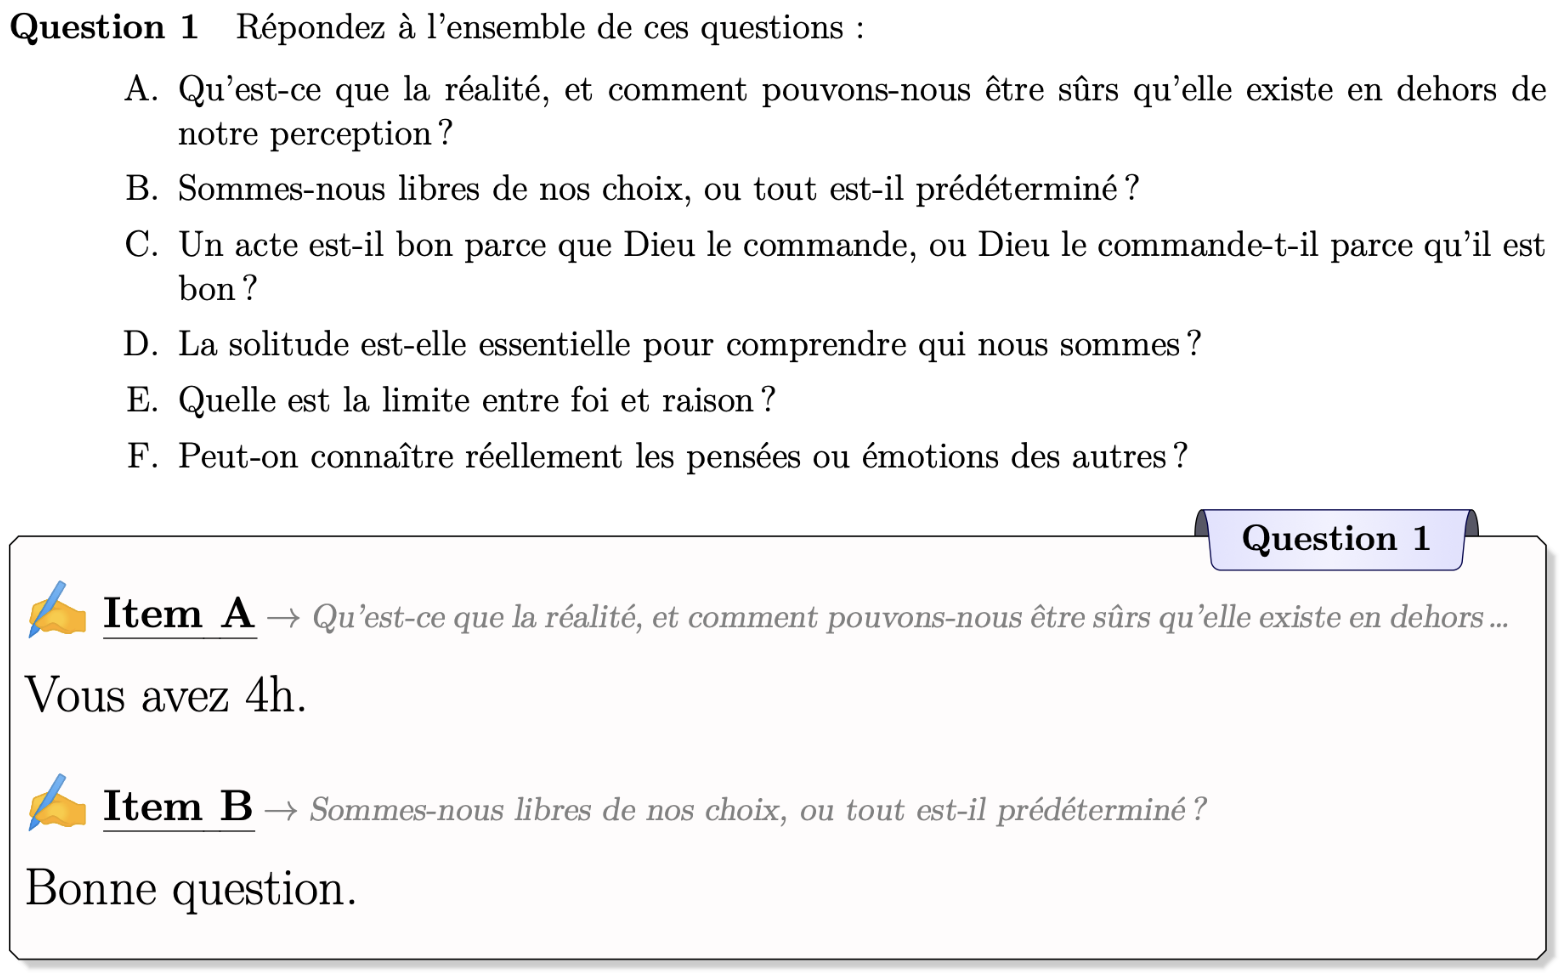
\includegraphics[width=0.8\linewidth]{img/correction.png}}
\end{center}

Notez qu'il est noté, en haut à droite de l'encadré, la question en cours de correction. Aussi, pour des questions ouvertes, l'émoji décorant \verb|\correctionitem| est \emoji{writing-hand}. Voir la section suivante \ref{correctionitem} pour découvrir les autres émojis.



\subsection{\texttt{\textbackslash correctionitem}}\label{correctionitem}

Cette commande doit \textbf{obligatoirement} se trouver au sein de l'environnement \verb|correction| ! Elle permet d'organiser davantage la correction, en déclarant quel(s) item(s) on souhaite corriger. En fonction des items donnés, \LaTeX{} sélectionnera un émoji de décoration conforme au bilan de réponse. En sachant que la commande s'appelle par exemple :

\begin{center}
    \verb|\correctionitem{Item A}|
\end{center}

Ou, autre exemple :

\begin{center}
    \verb|\correctionitem{Items A, B et E}|
\end{center}

Si l'on donne :

\begin{itemize}
    \item Un item vrai, la commande est décorée avec {\huge\raisebox{-3pt}{\textcolor{green!60!black}{\ding{52}}}}
    \item Un item faux, la commande est décorée avec {\huge\raisebox{-3pt}{\textcolor{red!90!black}{\ding{56}}}}
    \item Plusieurs items, la commande est décorée avec {\LARGE\mathversion{bold}\color{orange!95!black}\raisebox{-0pt}{\rotatebox{-15}{$?$}}\mathversion{normal}}
    \item Un item issu d'une question ouverte, la commande est décorée avec \emoji{writing-hand}
\end{itemize}

\bigskip

Inutile de gérer les espacements verticaux, \LaTeX{} se charge d'espacer suffisamment les différentes parties annoncées par \verb|\correctionitem|.

\begin{lstlisting}
\begin{correction}
    \correctionitem{Item A}
    <contenu>
    
    \correctionitem{Item B}
    <contenu>
    
    \correctionitem{Item C}
    <contenu>
    
    \correctionitem{Item D}
    <contenu>
    
    \correctionitem{Item E}
    <contenu>
\end{correction}
\end{lstlisting}


La commande \verb|\correctionitem|, lorsqu'elle prend en argument un seul item, fait le rappel de ce dernier. Mais si l'item est d'une structure complexe (item contenant une image par exemple), il est possible d'empêcher le rappel via la version étoilée \verb|\correctionitem*{Item X}|. A savoir que si l'item contient une image, et que la version étoilée n'est pas utilisée, la compilation mènera à des erreurs de type \texttt{LaTeX Error: Something's wrong--perhaps a missing \textbackslash item.}. 

\subsection{\texttt{\textbackslash verso}}

Cette commande ajoute, à la position où elle se trouve, la page de remerciement, soit le verso du support. Elle récupère toutes les informations nécessaires de l'environnement \verb|informations|. En sachant qu'on ne fera pas écho aux variables \verb|Relecteurs|, \verb|ConvertisseursLatex|, \verb|Testeurs|, \verb|TuteursEnSeance|, \verb|RemerciementsBonus|, si elles sont vides (intéressant quand on sait qu'il n'y a pas toujours de testeurs et compagnie).


\section{Autres fonctions A2SUP}

Abordons maintenant les quelques commandes et environnements annexes.


\subsection{Environnement \texttt{analyse}, \texttt{\textbackslash figanalyse} et \texttt{\textbackslash brouillon}}

L'environnement \texttt{analyse} est utilisé pour l'analyse de figures, comme c'est le cas en biologie cellulaire ou biochimie. Le contenu de cet environnement sera structuré à l'aide de deux autres commandes : \verb|\figanalyse{}| et \verb|\brouillon|. La première permet de séparer l'analyse des sous-figures composant la figure principale. La seconde permet de passer au brouillon que le rédacteur élabore au fur et à mesure du support.\\

A noter que l'environnement n'apparait que lorsque le support est une correction : évidemment, puisque l'analyse n'est à dévoiler que lors de la correction...

\begin{lstlisting}
\begin{analyse}
    \figanalyse{Figure 1A}
    La figure 1A est incroyable.

    \figanalyse{Figure 1B}
    Bangueur la team.

    \brouillon
    La figure $\rightarrow$ KliT
\end{analyse}
\end{lstlisting}

\begin{center}
    \fcolorbox{red!30}{red!30}{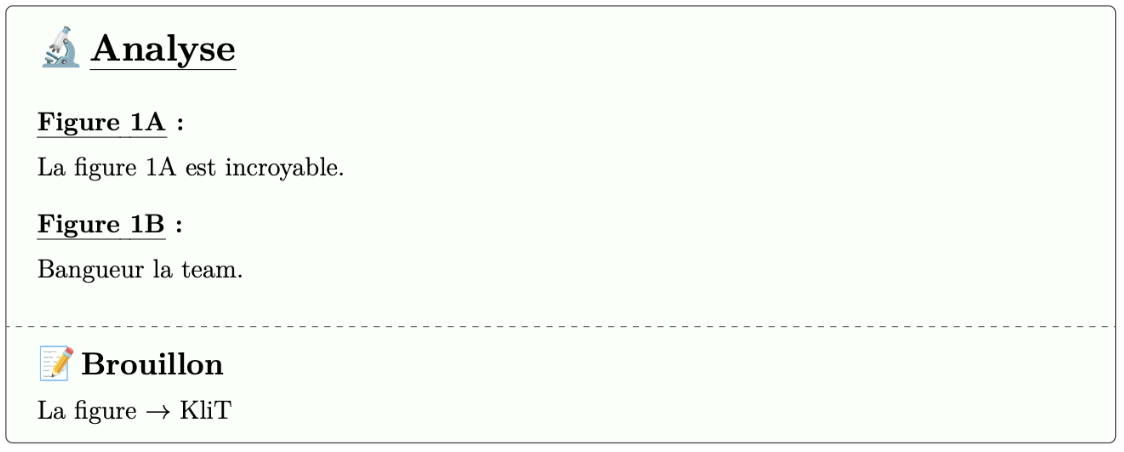
\includegraphics[width=0.7\linewidth]{img/analyse.png}}
\end{center}


\subsection{Environnement \texttt{boite}}\label{boite}

Cet environnement permet de mettre en évidence certaines informations, en les plaçant dans un encadré coloré. Il est souvent utilisé pour renforcer une notion à retenir. Mais libre à vous de l'utiliser selon vos besoins (tant que son utilisation reste raisonnable, l'objectif n'étant pas de transformer le support en une série de boites). Une boite peut se placer n'importe où dans le support.


\begin{lstlisting}
\begin{boite}
    <contenu de la boite>
\end{boite}
\end{lstlisting}

\begin{center}
    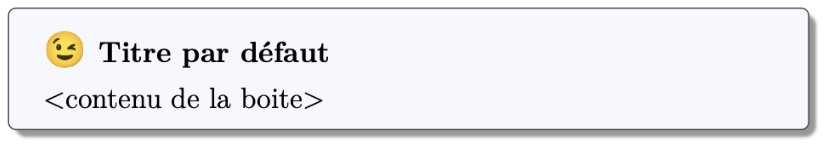
\includegraphics[width=0.85\linewidth]{img/boite_defaut.png}
\end{center}


Comme vous le voyez, il y a un émoji, un titre, une couleur et une largeur par défaut. 

\begin{itemize}
    \item émoji par défaut : \verb|\emoji{wink}|
    \item titre par défaut : "Titre par défaut"
    \item couleur par défaut : \verb|blue!3!white|
    \item largeur par défaut : \verb|0.85\linewidth|
\end{itemize}


\bigskip

Il est possible de personnaliser la boite :


\begin{lstlisting}
\begin{boite}[emoji=\emoji{heart}, titre=À retenir par cœur !, largeur=0.9\linewidth, couleur=green!1!white]
    L'intégrale de Gauss se résumé par l'égalité suivante :

    $$
    \int_\mathbb R e^{-x^2}\, dx = \pi
    $$
\end{boite}
\end{lstlisting}

\begin{center}
    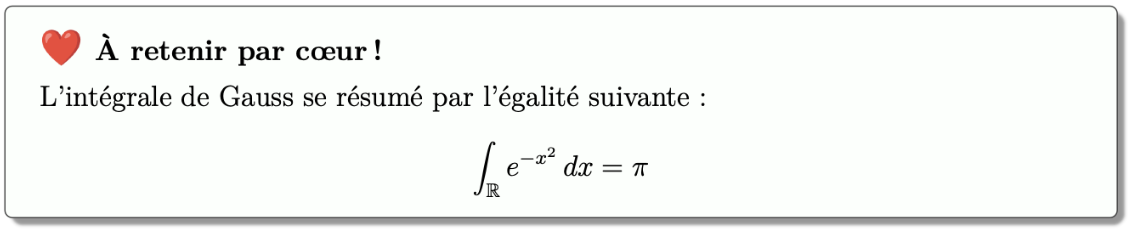
\includegraphics[width=0.9\linewidth]{img/boite.png}
\end{center}

Attention, je n'ai pas mis de \verb|{}| autour des valeurs, mais s'il y avait des virgules, j'aurais dû !


\subsection{\texttt{\textbackslash pagevide}}

Cette commande permet d'ajouter une page blanche (vide) à l'endroit où nous l'écrivons. La commande est cumulable : l'écrire 3 fois permettra d'ajouter 3 pages blanches.


\subsection{N'inclure que dans le sujet, ou que dans la correction}

L'environnement \verb|inclure| permet d'ajouter des éléments (environnement \verb|boite|, \verb|\pagevide|, des memes, etc) soit dans le sujet, soit dans la correction. Il peut particulièrement être utile pour les RM, qui doivent insérer des pages blanches pour obtenir un nombre paire de pages dans leur document final.

\begin{lstlisting}
\recto
\grille

\begin{inclure}[sujet]
    \pagevide
\end{inclure}

\begin{inclure}[correction]
    \pagevide
    \pagevide
\end{inclure}

\input{motRM}
\end{lstlisting}

Voici un cas fréquent : on ajoute 2 pages blanches dans la correction, et 1 page blanche dans le sujet.\\

\verb|\input{motRM}| ? La commande \verb|\input| permet d'intégrer du code présent dans un \textbf{autre} fichier .tex. Je recommande \textbf{très} fortement de mettre le mot des RM dans un fichier "motRM.tex", qui est ensuite appelé dans "main.tex" via \verb|\input{motRM}|. Le même raisonnement est applicable aux questions et exercices, voir section \ref{input}. L'intérêt est d'alléger les codes, pour les rendre plus lisibles.


\subsection{Questions et corrections dans un seul et même support}

Il peut arriver qu'on veuille poser des QCM d'entraînement, et dévoiler les réponses et corrections plus loin dans le support : c'est classiquement le cas dans les fiches de L.AS. Pour ce faire, on utilisera les mêmes commandes et environnements que tout à l'heure, avec une petite subtilité.\\

Nous utiliserons l'environnement \verb|memoire| ainsi que la commande \verb|reponse|.

\begin{itemize}
    \item L'environnement \verb|memoire| contiendra les questions et corrections de ces questions. L'environnement affichera ce contenu sous le paramètre \verb|sujet| (la correction ne sera donc pas affichée). L'affichage du sujet se fera à l'endroit où l'environnement est écrit.
    \item La commande \verb|reponse| libèrera de la mémoire les réponses, afin d'afficher cette fois le contenu mémoire, mais sous le paramètre \verb|correction|. L'affichage de la correction se fera à l'endroit où la commande est appelée.
\end{itemize}

\bigskip

Évidemment, \verb|\reponse| ne peut pas se situer en amont de l'environnement \verb|memoire|...

\begin{lstlisting}
\begin{memoire}
    \question{1}
    {Énoncé}
    {Item A}
    {Item B}
    {Item C}
    {Item D}
    {Item E}
    {AB}

    \begin{correction}
        \correctionitem{Items A, B, C, D et E}
        Trivial.
    \end{correction}

    \question{2}
    {Énoncé}
    {Item A de la question 2}
    {Item B de la question 2}
    {Item C de la question 2}
    {Item D de la question 2}
    {Item E de la question 2}
    {AB}

    \begin{correction}
        \correctionitem{Items A, B, C, D et E}
        Trivial encore une fois.
    \end{correction}
\end{memoire}


Faites le sujet avant de passer à la correction qui se touve juste en-dessous !

\reponse
\end{lstlisting}

\begin{center}
    \fcolorbox{red!30}{red!30}{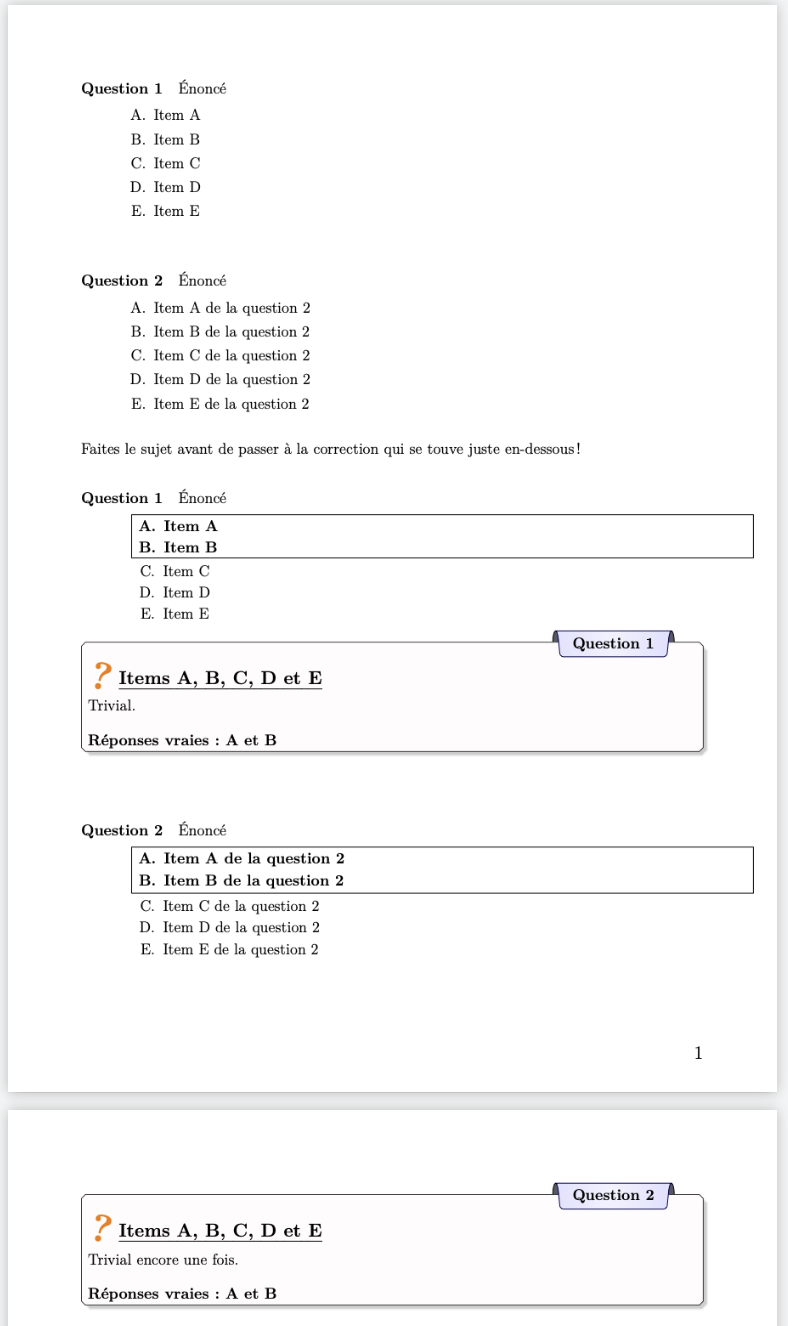
\includegraphics[height=0.8\paperheight]{img/memoire.png}}
\end{center}



Si besoin, il est possible de répéter environnement \verb|memoire| et \verb|\reponse| plusieurs fois. Chaque fois que l'environnement \verb|memoire| est appelé, la mémoire se rafraîchit, en écrasant l'ancienne. Il faut donc appeler la réponse avant.

\subsection{Solidariser un énoncé avec une question -- \texttt{\textbackslash inseparable}}

Comme dit dans le section \ref{Items}, les items et leur question ne peuvent être séparés par un saut de page. Ils sont solidaires. Il est possible de solidariser à cette ensemble, tout ou partie d'un énoncé. Il suffit de placer la commande \verb|\inseparable| en amont de la partie d'énoncé à solidariser.

\begin{lstlisting}
Paragraphe n°1\\

Paragraphe n°2

\inseparable

Paragraphe n°3

\question{1}
{Énoncé}
{Item A}
{Item B}
{Item C}
{Item D}
{Item E}
{AE}
\end{lstlisting}

Ainsi, le paragraphe n°3 sera toujours sur la même page que la question suivante. Cela permet aux p1 de ne pas faire des allers-retours chronophages et déstabilisants entre deux pages pour répondre à une question à partir de données de l'énoncé.\\

\verb|\inseparable| peut prendre une option : \verb|\inseparable[sujet]| ne sera effective que dans le sujet, \verb|\inseparable[correction]| ne sera effective que dans la correction, et, par défaut, \verb|\inseparable[toujours]|, donc inutile de préciser l'option "toujours" si la valeur par défaut convient.


\subsection{Ajouter une annexe}\label{annexe}

Dans certaines UEs comme les Mathématiques, une annexe est nécessaire dans le support (de tuto). La commande \verb|\annexe| a été créée à cet effet.

\begin{lstlisting}
    \annexe      OU      \annexe[nom_du_pdf]
\end{lstlisting}

Cette commande n'a qu'1 seul argument optionnel. Sans l'argument optionnel, \LaTeX{} part du principe que votre annexe s'appelle "annexe.pdf", et qu'il est présent dans votre projet. Sinon, il ira chercher le pdf du nom indiqué. À savoir que l'annexe ne sera pas paginée, et que la pagination sera en pause sur l'étendue de l'annexe : le nombre total de pages indiqué par \LaTeX{} (et affichée sur la page de couverture pour un tuto ou une annale) ne tiendra pas compte du nombre de pages dans l'annexe.\\

En Mathématiques, l'annexe arrive après la page de remerciements, et uniquement dans la version sujet, comme ceci :

\begin{lstlisting}
\verso 

\begin{inclure}[sujet]
    \annexe
\end{inclure}
\end{lstlisting}

Mais libre à vous de l'afficher en début de support, dans le sujet, ou dans la correction, ou dans les deux.


\section{Commandes utiles externes à \texttt{A2SUP.sty}}

Voici un certain nombre de commandes issues d'autres packages, mais très utiles.

\subsection{Tableaux avec \texttt{tabular} ou \texttt{tabularx}}\label{tableaux}

Je vous renvoie vers \url{https://www.overleaf.com/learn/latex/Tables} pour en savoir plus sur l'environnement \verb|tabular|. Je note pour information qu'il ne faut pas utiliser l'environnement \verb|table| !! Cet environnement est utile pour des document très rédactionnels comme des thèses ou des articles scientifiques, mais il est très embêtant à utiliser dans un document contenant une variété de contenus. Notamment, il ne place pas les images là où l'on souhaite vraiment les placer, avec les espacements adéquats\footnote{Même avec la fameuse option \texttt{[h!]} je vous assure.}.\\

L'environnement \verb|tabularx| présente une différence par rapport à \verb|tabular|, résidant dans le fait qu'on peut plus facilement déterminer la largeur du tableau directement, sans devoir calculer la largeur de chaque colonne, déterminant alors indirectement la largeur du tableau. En effet, alors qu'un tableau \verb|tabular| sera codé comme ceci :

\begin{lstlisting}
\begin{tabular}{|c|c|}
    \hline
        A & B \\
    \hline
        1 & 2 \\
    \hline
\end{tabular}
\end{lstlisting}


Un tableau \verb|tabularx| sera codé comme cela, en supposant que l'on veuille un tableau occupant 80\% de la largeur de la page :

\begin{lstlisting}
\begin{tabularx}{0.8\linewidth}{|c|X|}
    \hline
        A & B \\
    \hline
        1 & 2 \\
    \hline
\end{tabularx}
\end{lstlisting}

On remarque que :

\begin{itemize}
    \item le nom de l'environnement est passé de \verb|tabular| à \verb|tabularx|
    \item L'environnement a un argument supplémentaire \verb|{0.8\linewidth}|, déterminant la largeur (et uniquement la largeur) du tableau
    \item un argument de position \verb|c| donne \verb|X|
    \item en compilant ce tableau, les éléments de la deuxième position ne sont plus centrés
\end{itemize}

L'argument de position \verb|X| signifie que, sur les 80\% de la largeur de la page, l'espace n'étant pas occupée par la première colonne sera entièrement occupée par la deuxième colonne.\\

Cependant, je peux avoir envie de lui donner tout l'espace restant, tout en centrant le contenu. Dans ce cas, je mets non pas \verb|X|, mais \verb|>{\centering\arraybackslash}X|.\\

Et si j'ai envie d'aligner, en plus de l'axe horizontal, verticalement ? J'ajoute, avant l'environnement \verb|tabularx|, la ligne \verb|\renewcommand\tabularxcolumn[1]{m{#1}}|\footnote{\url{https://tex.stackexchange.com/questions/343028/vertical-centering-of-all-columns-in-tabularx-environment}}


\begin{lstlisting}
\renewcommand{\arraystretch}{1.5}
\renewcommand\tabularxcolumn[1]{m{#1}}
\begin{tabularx}{0.8\linewidth}{|c|>{\centering\arraybackslash}X|}
    \hline
        A & B \\
    \hline
        1 & 2 \\
    \hline
\end{tabularx}
\end{lstlisting}

En sachant que je peux parfaitement allouer l'argument de position \verb|X| à autant de colonnes que je souhaite : je diviserai simplement autant de fois que nécessaire l'espace restant (2 fois si deux colonnes ont cet argument par exemple).\\

\verb|\renewcommand{\arraystretch}{1.5}| permet d'augmenter l'espacement vertical dans le tableau. La valeur de 1.5 signifie que j'étire de 50\% la ligne basale en verticalité. Si un espace unitaire mesurait initialement 1 cm de haut, il mesurera alors 1.5 cm. Cette explication n'est que du détail, mais ça peut vous être utile quand vous souhaitez optimiser la valeur de \verb|\arraystretch|.



\subsection{\texttt{\textbackslash input}}

Cette commande est indispensable si l'on veut un projet agréable à reprendre de tous ! En résumé, cette commande permet de relier un fichier .tex à un autre fichier .tex.\\

Quand un support est rédigé, le fichier utilisé est \verb|main.tex|. Mais quand on sait que, par exemple, les mathématiques sont organisées en 3 exercices généralement, on ne va pas surcharger ce fichier en y mettant la longue rédaction des exercices. À la place, dans le projet, on peut créer un dossier \verb|Exercices|, dans lequel on place trois fichiers \verb|Exercice 1.tex|, \verb|Exercice 2.tex| et \verb|Exercice 3.tex|, contenant chacun les rédactions des exercices respectifs. On n'a plus qu'à informer \LaTeX{}, dans \verb|main.tex|, que l'exercice 1 se trouve dans \verb|Exercice 1.tex|, etc.

\begin{center}
    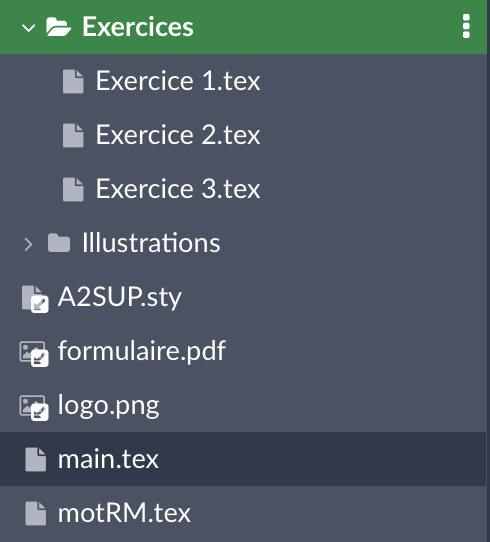
\includegraphics[height=4.5cm]{img/orga_simple.png} \, 
    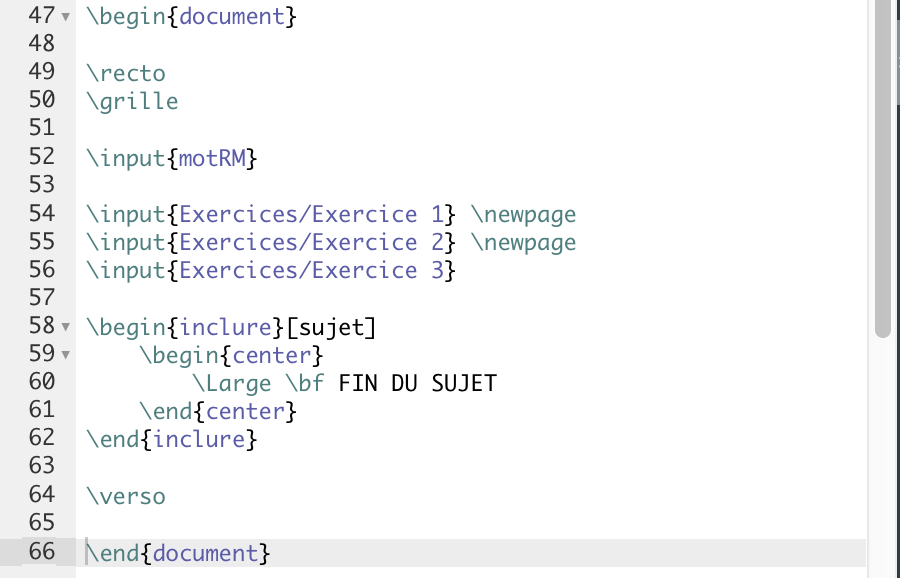
\includegraphics[height=4.5cm]{img/codes_simples.png}
\end{center}


Et là, tout devient beaucoup plus visuel ! On sait directement comment est structuré le document : en premier vient le recto, puis la grille, puis le mot des RM (dont le contenu se trouve dans le fichier \verb|motRM.tex|), puis les trois exercices (en faisant un saut de page entre chaque exercice), puis un indicatif de fin de sujet, et, enfin, un verso. Cette organisation est très pratique, car \verb|main.tex| a plus le rôle de "chef d'orchestre". Il décide d'intégrer tel ou tel élément : il suffit de commenter \footnote{\textsl{\texttt{contrôle /} sur Windows ou \texttt{command /} sur Mac}. N'hésitez pas à consulter les nombreux raccourcis clavier sur Overleaf sur \url{https://www.overleaf.com/articles/overleaf-keyboard-shortcuts/qykqfvmxdnjf}} la ligne 54 si je ne veux pas compiler l'exercice 1 (et non TOUTES les lignes de cet exercice...) !


C'est aussi très pratique pour ceux qui souhaitent exploiter le projet plus tard (notamment pour les annales, comme c'est le cas pour ce projet), mais aussi pour des futurs RMs ayant la volonté de piocher dans les anciens sujets pour compiler, par exemple, un polycopié d'exercices en plus, pour fournir plus de supports aux P1. Tout devient plus facile, puisqu'on sait exactement où chercher. Noter aussi que les images sont toutes dans un même dossier, ici nommé \verb|Illustrations| (consensus pour les annales, donc si vous voulez simplement recopier ce consensus, alors aucun soucis, que du bonheur)\footnote{À noter que le formulaire ici s'appelle formulaire, mais aurait dû s'appeler \texttt|annexe.pdf| en toute rigueur (voir section \ref{annexe}), mais puisqu'on ne l'insère pas dans les sessions d'annales, j'avoue être passé à côté... ou bien, je pourrais appeler non pas \texttt{\textbackslash annexe} mais \texttt{\textbackslash annexe[formulaire]} \emoji{smile}}.


\newpage

\subsection{\texttt{\textbackslash includegraphics pour ajouter des images}}

Cette commande permet d'ajouter une image, sous format \verb|png|, \verb|jpeg|, \verb|jpg|, et même \verb|pdf| !\footnote{Très utile pour un trick que je développerai prochainement, notamment en chimie et physique.}.\\

Voici les étapes pour ajouter une image :

\begin{itemize}
    \item Ajouter l'image dans le projet, dans le dossier \verb|Illustrations|, ou équivalent si existant, en le nommant, par exemple "une-image.png"
    \item À l'endroit désiré, si je veux la centrer, et lui donner une légende, 
    \begin{lstlisting}
\begin{center}
    \includegraphics[width=0.5\linewidth]{Illustrations/une-image.png}

    Une légende
\end{center}
    \end{lstlisting}
    \item Ajuster la largeur si besoin
\end{itemize}

Les options utilisables sont :

\begin{itemize}
    \item \verb|width| : largeur, en longueur relative (\verb|0.3\linewidth|) ou absolue (\texttt{2cm})
    \item \verb|height| : hauteur, en longueur relative (\verb|0.3\paperheight|) ou absolue (\texttt{2cm})
    \item angle : rotation dans le sens inverse des aiguilles, en degrés (\verb|angle=45| fera tourner l'image de 45° dans le sens inverse des aiguilles)
\end{itemize}

Je déconseille très fortement d'utiliser \verb|scale|, car la valeur que vous lui assignez dépend énormément des propriétés directes de l'image : l'image peut être très petite, ce qui nécessitera une grande échelle ; l'image peut être grande, ce qui nécessitera une petite échelle. Ce n'est donc pas la variable la plus directe à utiliser, puisque ce qui nous intéresse essentiellement, est la dimension de l'image au sein de notre page. Il est donc plus cohérent de comparer la largeur (ou la hauteur) de notre image à la largeur (ou la hauteur) de notre page.\\

Pour revenir à l'étape de l'importation d'une image sur Overleaf, il existe une manipulation assez rapide. Voici le tutoriel vidéo : \url{https://shorturl.at/gKPgc}. Remarquez que le copier-coller ne fonctionne pas lorsque l'image se trouve dans un GDoc. La raison est que Google empêche le collage d'une image dans une source externe à Google lorsque l'image provient d'une extension de Google Drive (GDoc, GSheet, GSlides...). Il faudra donc télécharger le fichier en Word, et manipuler ce dernier fichier.

\subsection{Titres, sous-titres et sous-sous-titres -- Sommaire}

Il est parfois souhaité d'organiser le PDF en parties : 3 exercices pour un tuto de mathématiques ; une structure plus complexe pour une fiche d'histologie... Voici comment cela fonctionne :

\begin{lstlisting}
\tableofcontents

\hrule

\section{Partie 1 : Introduction}

\subsection{Sous-partie 1 : Contexte}

Blabla.

\subsection{Sous-partie 2 : Problématiques}

Blabla.

\subsubsection{Sous-sous partie 1 : Questions}

Bla.

\section{Partie 2 : Péripéties}

Bla.
\end{lstlisting}

\verb|\tableofcontents| permet d'obtenir le sommaire (table des matières) et je scinde visuellement les deux parties du document avec \verb|\hrule|, qui trace un trait sur la largeur de la page : 

\begin{center}
    \fcolorbox{red!30}{red!30}{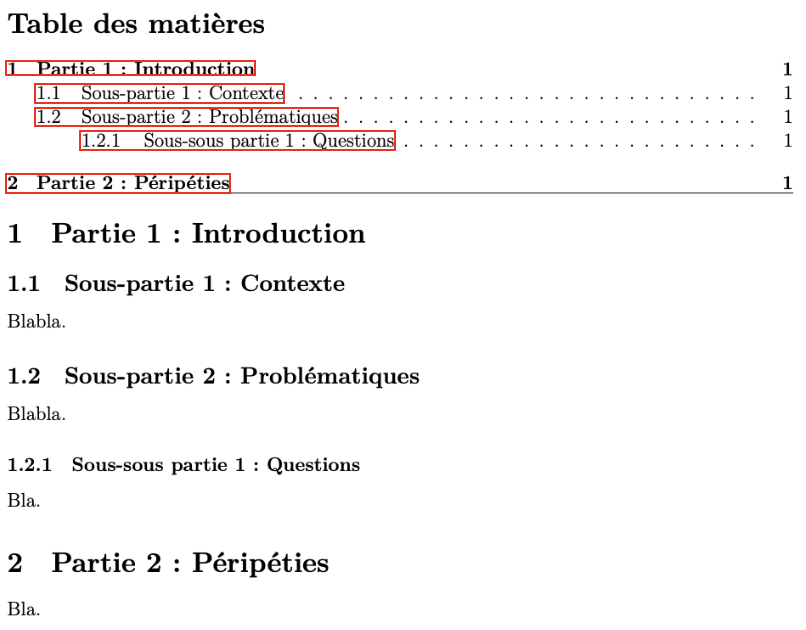
\includegraphics[width=0.6\linewidth]{img/sections.png}}
\end{center}


Il est possible de retirer la numérotation des sections, en utilisant la version \texttt{*} des commandes : \verb|\section*{}|, \verb|\subsection*{}|, \verb|\subsubsection*{}|

\begin{lstlisting}
\tableofcontents

\hrule

\section*{Partie 1 : Introduction}

\subsection*{Sous-partie 1 : Contexte}

Blabla.

\subsection*{Sous-partie 2 : Problématiques}

Blabla.

\subsubsection*{Sous-sous partie 1 : Questions}

Bla.

\section*{Partie 2 : Péripéties}

Bla.
\end{lstlisting}

\begin{center}
    \fcolorbox{red!30}{red!30}{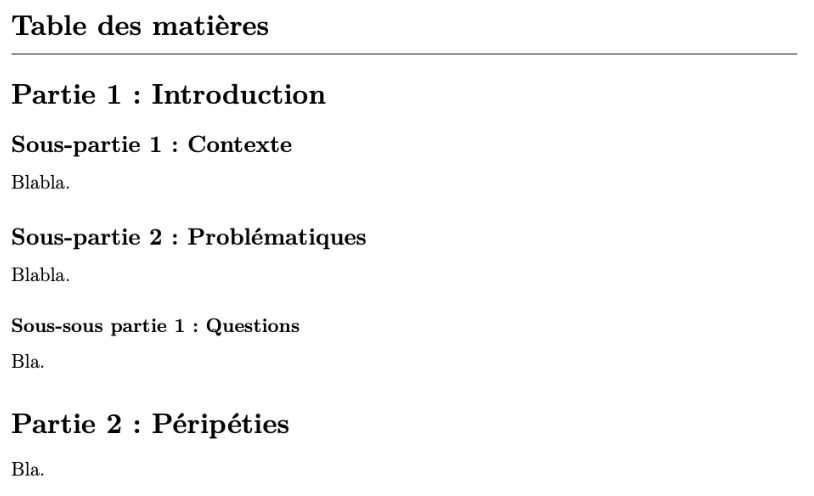
\includegraphics[width=0.6\linewidth]{img/sections non numérotées.png}}
\end{center}

Vous remarquez que le sommaire est vide ! Pour ajouter dans le sommaire des sections étoilées, il est nécessaire d'ajouter la ligne \verb|\addcontentsline{toc}{<sub><sub>section}{<TITLE>}| : il faudra préciser s'il est question d'une \textsl{section}, d'une \textsl{subsection} ou d'une \textsl{subsubsection}, ainsi que le nom de la section, comme ceci,


\begin{lstlisting}
\tableofcontents

\hrule

\addcontentsline{toc}{section}{Partie 1 : Introduction}
\section*{Partie 1 : Introduction}

\addcontentsline{toc}{subsection}{Sous-partie 1 : Contexte}
\subsection*{Sous-partie 1 : Contexte}

Blabla.

\addcontentsline{toc}{subsection}{Sous-partie 2 : Problématiques}
\subsection*{Sous-partie 2 : Problématiques}

Blabla.

\addcontentsline{toc}{subsubsection}{Sous-sous partie 1 : Questions}
\subsubsection*{Sous-sous partie 1 : Questions}

Bla.

\addcontentsline{toc}{section}{Partie 2 : Péripéties}
\section*{Partie 2 : Péripéties}

Bla.
\end{lstlisting}


\begin{center}
    \fcolorbox{red!30}{red!30}{\includegraphics[width=0.6\linewidth]{img/sections non paginées dans sommaire.png}}
\end{center}


Enfin, si la mise en page vous semble trop peu joyeuse, il est possible d'y ajouter de la couleur, en donnant l'option \verb|plan=oui| lors de l'importation du package \verb|A2SUP| (voir section \ref{Importation}).


\begin{lstlisting}
\usepackage[plan=oui]{A2SUP}

...

\tableofcontents

\hrule

\addcontentsline{toc}{section}{Partie 1 : Introduction}
\section*{Partie 1 : Introduction}

\subsection*{Sous-partie 1 : Contexte}

Blabla.

\subsection*{Sous-partie 2 : Problématiques}

Blabla.

\subsubsection*{Sous-sous partie 1 : Questions}

Bla.

\section*{Partie 2 : Péripéties}

Bla.
\end{lstlisting}

\begin{center}
    \fcolorbox{red!30}{red!30}{\includegraphics[width=0.6\linewidth]{img/sections colorées.png}}
\end{center}


Je ne le montre pas ici, mais il est possible d'appliquer ces couleurs, tout en retirant la numérotation !




\subsection{Couleur de texte}

Puis nous avons abordé les couleurs, voyons comment exploiter les couleurs dans les textes. Il existe plusieurs façons de déterminer la couleur d'une lettre, d'un mot, d'un groupe de mots, ou d'un paragraphe. À mon sens, la plus directe et la plus généralisable est celle-ci :

\begin{lstlisting}
Le texte est noir actuellement, mais {\color{red!70!black} je peux le rendre
rouge}. Et ce, temporairement...

$$
1+1 {\color{purple} \ne} 2
$$
\end{lstlisting}

\fcolorbox{red!30}{red!30}{\begin{minipage}{\dimexpr\linewidth-2\fboxsep\relax}
Le texte est noir actuellement, mais {\color{red!70!black} je peux le rendre rouge}. Et ce, temporairement...

$$
1+1 {\color{purple} \ne} 2
$$
\end{minipage}}

\medskip

Placer du contenu entre \verb|{}| permet de créer un \textsl{espace} différent, dans lequel on peut définir des propriétés de mise en page, notamment \verb|\color{purple}| ici. Mais ce n'est pas tout !

\begin{lstlisting}
Un texte avec un {\color{blue}\sl\bfseries mot} différent.
\end{lstlisting}

\fcolorbox{red!30}{red!30}{Un texte avec un {\color{blue}\sl\bfseries mot} différent.}

\subsection{Mise en gras, italique, soulignage}\label{stylisation}

Comme dans le section précédente, on peut appliquer du gras en créant un espace à part via \verb|{}|. Mais ce n'est pas la seule façon pour mettre du texte en gras : 

\begin{lstlisting}
Je veux du {\bfseries gras} pour un mot uniquement.\\

Je veux encore une fois du \textbf{gras} pour un mot.

\bigskip

\begin{bfseries}
    Cette fois, je veux qu'un grand nombre de mots soit mis en gras. J'utilise
    l'environnement pour ne pas avoir des \{\} distants les unes des autres, ce
    qui est peu lisible et source d'erreurs faciles si j'oublie de fermer une
    accolade.
\end{bfseries}
\end{lstlisting}


\fcolorbox{red!30}{red!30}{\begin{minipage}{\dimexpr\linewidth-2\fboxsep\relax}
    Je veux du {\bfseries gras} pour un mot uniquement.\\

    Je veux encore une fois du \textbf{gras} pour un mot.

    \bigskip
    
    \begin{bfseries}
        Cette fois, je veux qu'un grand nombre de mots soit mis en gras. J'utilise l'environnement pour ne pas avoir des \{\} très distants les uns des autres, ce qui est peu lisible et source d'erreurs faciles si j'oublie de fermer une accolade.
    \end{bfseries}
\end{minipage}}

\medskip

Sur Overleaf, le raccourci clavier \verb|Contrôle B| (\verb|Command B| avec Apple) sur la sélection met la sélection en gras via \verb|\textbf|.\\

Pour la mise en italique, le raccourci clavier est \verb|Contrôle I| (\verb|Command I| avec Apple), et donne la commande \verb|\textit|. Néanmoins, la mise en italique via cette commande n'est pas très esthétique je trouve, donc je recommande ces codes :

\begin{lstlisting}
Je veux de {\slshape l'italique} pour un mot uniquement.\\

Voici en comparaison, de {\itshape l'italique} pas très esthétique.\\

Je veux encore une fois de l'\textsl{italique} pour un mot.

\bigskip

\begin{slshape}
    Cette fois, je veux qu'un grand nombre de mots soit mis en italique. 
    J'utilise l'environnement pour ne pas avoir des \{\} très distants les uns 
    des autres, ce qui est peu lisible et source d'erreurs faciles si j'oublie 
    de fermer une accolade.
\end{slshape}
\end{lstlisting}

\fcolorbox{red!30}{red!30}{\begin{minipage}{\dimexpr\linewidth-2\fboxsep\relax}
    Je veux de {\slshape l'italique} pour un mot uniquement.\\

    Voici en comparaison, de {\itshape l'italique} pas très esthétique.\\
    
    Je veux encore une fois de l'\textsl{italique} pour un mot.
    
    \bigskip
    
    \begin{slshape}
        Cette fois, je veux qu'un grand nombre de mots soit mis en italique. J'utilise l'environnement pour ne pas avoir des \{\} très distants les uns des autres, ce qui est peu lisible et source d'erreurs faciles si j'oublie de fermer une accolade.
    \end{slshape}
\end{minipage}}

\medskip

Pour conclure, le soulignage se fait via une seule commande : \verb|\uline{}|\footnote{Vous pourrez tomber sur la commande \texttt{\textbackslash underline\{\}}, mais elle présente l'inconvénient de ne pas souligner sur plus d'une ligne. Aussi, elle ne souligne pas les mots de la même façon, ce qui rend le visuel pas très homogène : 

\begin{itemize}
    \item \underline{mot}, \underline{parfait}, \underline{ligne}, \underline{colonne} ; avec \texttt{\textbackslash underline}
    \item \uline{mot}, \uline{parfait}, \uline{ligne}, \uline{colonne} ; avec \texttt{\textbackslash uline}
\end{itemize}

Donc il est préférable d'utiliser \texttt{\textbackslash uline\{\}} systématiquement.}. Si vous consultez le package \verb|ulem|, via \url{https://texdoc.org/serve/ulem/0}, vous verrez qu'il est possible de \uuline{souligner} \uwave{différemment} \dotuline{vos contenus}, et même de \xout{raturer du texte} !\\

Évidemment il est possible de combiner les styles de texte :

\begin{lstlisting}
\uline{Ceci est une phrase soulignée, contenant \textbf{une partie en gras}, et \textsl{une partie en italique}, en notant qu'on peut ajouter {\color{blue}\bfseries\slshape une troisième partie en gras, italique, et colorée}}.
\end{lstlisting}

\fcolorbox{red!30}{red!30}{\begin{minipage}{\dimexpr\linewidth-2\fboxsep\relax}
    \uline{Ceci est une phrase soulignée, contenant \textbf{une partie en gras}, et 
    \textsl{une partie en italique}, en notant qu'on peut ajouter {\color{green!70!black}
    \bfseries\slshape une troisième partie en gras, italique, et colorée}}.
\end{minipage}}

\subsection{Modifier la taille de police}


Si vous avez bien compris la notion d'espace créé via l'utilisation de \verb|{}|, alors vous comprendrez comment on modifie la taille de police de tout ou partie d'un texte, en sachant que les environnements existent aussi, de la même façon que la stylisation du texte qu'on étudie dans la section précédente (section \ref{stylisation}).

\begin{lstlisting}
Voici un texte contenant un {\tiny très petit mot}. En voici un {\huge très 
grand}, voire encore {\Huge plus grand}.

\bigskip

\begin{footnotesize}
    Voici un paragraphe que je veux écrire un petit, mais suffisamment grand 
    pour que ce soit agréable à lire.
\end{footnotesize}
\end{lstlisting}

\fcolorbox{red!30}{red!30}{\begin{minipage}{\dimexpr\linewidth-2\fboxsep\relax}
    Voici un texte contenant un {\tiny très petit mot}. En voici un {\huge très grand}, voire encore {\Huge plus grand}.
    
    \bigskip
    
    \begin{footnotesize}
        Voici un paragraphe que je veux écrire un petit, mais suffisamment grand pour que ce soit agréable à lire.
    \end{footnotesize}
\end{minipage}}



\subsection{Emojis}

Il est possible d'utiliser des émojis en exploitant le package \verb|emoji| : \url{https://ctan.math.washington.edu/tex-archive/macros/luatex/latex/emoji/emoji-doc.pdf}. C'est, entre autres, pour ce package qu'on utilise Lua\LaTeX.\\

Il faut utiliser les noms donnés dans les colonnes \verb|Fullname| et \verb|Aliases|.



\subsection{Puçages et listes}

Il est possible de faire des listes de deux manières différentes, en fonction de si l'on veut numéroter ou non la liste. Si la liste n'est pas numérotée, nous utilisons l'environnement \verb|itemize|. Si la liste est numérotée, nous utilisons l'environnement \verb|enumitem|.

\subsubsection{Listes non numérotées}

\begin{lstlisting}
Voici une liste :

\begin{itemize}
    \item Un premier item
    \item Un deuxième item
\end{itemize}

\medskip

J'en ai terminé avec ma liste !
\end{lstlisting}

\fcolorbox{red!30}{red!30}{\begin{minipage}{\dimexpr\linewidth-2\fboxsep\relax}
    Voici une liste :

    \begin{itemize}
        \item Un premier item
        \item Un deuxième item
    \end{itemize}
    
    \medskip
    
    J'en ai terminé avec ma liste !
\end{minipage}}

\medskip

Remarquez qu'il n'y a aucun \verb|\\| ! Il n'est pas correct d'en utiliser dans ce contexte, comme dans tout contexte d'environnement. Pour espacer avec le paragraphe arrivant après la liste, j'ai posé \verb|medskip|, je peux réduire l'espacement vertical avec \verb|\smallskip|, ou l'augmenter via \verb|\bigskip|.\\

Si vous trouvez que la mise en page n'est pas intéressante pour les listes, vous pouvez décider de choisir le label des items !

\begin{lstlisting}
Voici une première liste avec un label dont je détermine le type, la taille et la couleur :

\begin{itemize}[label=$\bullet$, font=\small\color{blue}]
    \item Un premier item
    \item Un deuxième item
\end{itemize}

\medskip

Voici une deuxième liste dans laquelle les items ont pour label un émoji :

\begin{itemize}[label=\emoji{tr}]
    \item Un premier item
    \item Un deuxième item
\end{itemize}
\end{lstlisting}

\fcolorbox{red!30}{red!30}{\begin{minipage}{\dimexpr\linewidth-2\fboxsep\relax}
    Voici une première liste avec un label dont je détermine le type, la taille et la couleur :
    
    \begin{itemize}[label=$\bullet$, font=\small\color{blue}]
        \item Un premier item
        \item Un deuxième item
    \end{itemize}
    
    \medskip
    
    Voici une deuxième liste dans laquelle les items ont pour label un émoji :
    
    \begin{itemize}[label=\emoji{tr}]
        \item Un premier item
        \item Un deuxième item
    \end{itemize}
\end{minipage}}



\subsubsection{Listes numérotées}

Cette fois, on utilise l'environnement \verb|enumerate| pour une liste organisée :

\begin{lstlisting}
Voici une liste organisée :

\begin{enumerate}
    \item Le premier item
    \item Le deuxième item
\end{enumerate}

\medskip

Et voila ! Maintenant, je veux une liste ordonnée avec des chiffres romains, suivis d'un tiret : 

\begin{enumerate}[label=\Alph* -]
    \item Le premier item
    \item Le deuxième item
\end{enumerate}
\end{lstlisting}


\fcolorbox{red!30}{red!30}{\begin{minipage}{\dimexpr\linewidth-2\fboxsep\relax}
    Voici une liste organisée :

    \begin{enumerate}
        \item Le premier item
        \item Le deuxième item
    \end{enumerate}
    
    \medskip
    
    Et voila ! Maintenant, je veux une liste ordonnée avec des chiffres romains, suivis d'un tiret : 

    \begin{enumerate}[label=\Roman* -]
        \item Le premier item
        \item Le deuxième item
    \end{enumerate}
\end{minipage}}

\bigskip

En sachant que :

\begin{itemize}
    \item \verb|label=\Alph*| : lettres majuscules
    \item \verb|label=\alph*| : lettres minuscules
    \item \verb|label=\Roman*| : chiffres romains majuscules
    \item \verb|label=\roman*| : chiffres romains minuscules
    \item \verb|label=\arabic*| : chiffres arabes
\end{itemize}


\subsection{Listes imbriquées}


Maintenant que vous savez tout, nous pouvons imbriquer les listes les unes dans les autres :

\begin{lstlisting}
\begin{itemize}[label=\emoji{backhand-index-pointing-right-dark-skin-tone}]
    \item Turquie :
        \begin{itemize}[label=\textbullet, font=\small]
            \item 3 lieux à ne pas rater :
                \begin{enumerate}[font=\color{red}]
                    \item Istanbul
                    \item Cappadoce
                    \item Bursa
                \end{enumerate}
            \item 85 millions d'habitants
            \item 783 562 km\up{2}
        \end{itemize}
    \item France :
        \begin{itemize}[label=\textbullet, font=\small]
            \item 3 lieux à ne pas rater :
                \begin{enumerate}[font=\color{red}]
                    \item Paris
                    \item Le Mont Saint-Michel
                    \item La Côte d'Azur
                \end{enumerate}
            \item 68 millions d'habitants
            \item 551 695 km\up{2}
        \end{itemize}
\end{itemize}
\end{lstlisting}

\fcolorbox{red!30}{red!30}{\begin{minipage}{\linewidth}
    \begin{itemize}[label=\emoji{backhand-index-pointing-right-dark-skin-tone}]
        \item Turquie :
            \begin{itemize}[label=\textbullet, font=\small]
                \item 3 lieux à ne pas rater :
                    \begin{enumerate}[font=\color{red}]
                        \item Istanbul
                        \item Cappadoce
                        \item Bursa
                    \end{enumerate}
                \item 85 millions d'habitants
                \item 783 562 km\up{2}
            \end{itemize}
        \item France :
            \begin{itemize}[label=\textbullet, font=\small]
                \item 3 lieux à ne pas rater :
                    \begin{enumerate}[font=\color{red}]
                        \item Paris
                        \item Le Mont Saint-Michel
                        \item La Côte d'Azur
                    \end{enumerate}
                \item 68 millions d'habitants
                \item 551 695 km\up{2}
            \end{itemize}
    \end{itemize}
\end{minipage}}








\subsection{Inclure des liens cliquables}

Un lien cliquable peut être ajouté à l'aide de deux commandes différentes : \verb|\url{}| et \verb|\href{}{}|.\\

\verb|\url{}| ajoute le lien en l'affichant de façon brute.

\begin{lstlisting}
\url{https://www.youtube.com/watch?v=ZKCQP2DfkPk}
\end{lstlisting}

\fcolorbox{red!30}{red!30}{\url{https://www.youtube.com/watch?v=ZKCQP2DfkPk}}

\bigskip

Mais il se peut que vous n'ayez pas envie d'afficher le lien, car trop long ou pas très beau. Dans ce cas, vous pouvez le lien à un nom cliquable :

\begin{lstlisting}
\href{https://www.youtube.com/watch?v=ZKCQP2DfkPk}{Comment devenir un.e beau/belle gauss ?}
\end{lstlisting}

\fcolorbox{red!30}{red!30}{\href{https://www.youtube.com/watch?v=ZKCQP2DfkPk}{Comment devenir un.e beau/belle gauss ?}}

\bigskip

Attention néanmoins, mettre un lien dans un nom, c'est prendre le risque que les P1 travaillant sur la version papier ne prennent pas le temps de retrouver le support numérique pour cliquer sur le lien cliquable (encore faut-ils le sachant. En version numérique, les liens cliquables sont encadrés par \LaTeX{}). Donc si vous avez un lien trop long, n'hésitez pas à le raccourcir sur \url{https://www.shorturl.at}, site qui raccourcit les liens sans aucune date de péremption !


\subsection{Écrire des calculs}


\subsubsection{Modes \textsl{inline} et \textsl{math}}

Les calculs mathématiques passent par l'utilisation de \verb|$|. Il faut distinguer deux modes mathématiques : 

\begin{description}
    \item[Mode inline :] Il permet d'incruster des maths dans un texte\\
        \begin{lstlisting}
J'ai 2 bonbons, on m'en pique un. Il ne m'en reste plus que $2-1=1$.
        \end{lstlisting}
        \fcolorbox{red!30}{red!30}{\begin{minipage}{\dimexpr\linewidth-2\fboxsep\relax}
            J'ai 2 bonbons, on m'en pique un. Il ne m'en reste plus que $2-1=1$ !
        \end{minipage}}

    \item[Mode math :] Il formate les calculs dans un paragraphe à part entière, en dehors de paragraphes textuels. Une particularité est que le calcul écrit sera centré, et espacé verticalement, comme le serait un environnement. \textbf{On n'utilise donc pas de \texttt{\textbackslash\textbackslash} pour sauter des lignes !}\\
        \begin{lstlisting}
J'ai 2 bonbons, on m'en pique un. Voici ce qu'il me reste :

$$
2-1=1
$$

Je n'ai donc plus qu'un seul bonbon !
        \end{lstlisting}
        \fcolorbox{red!30}{red!30}{\begin{minipage}{\dimexpr\linewidth-2\fboxsep\relax}
            J'ai 2 bonbons, on m'en pique un. Voici ce qu'il me reste :

            $$
            2-1=1
            $$

            Je n'ai donc plus qu'un seul bonbon !
        \end{minipage}}
\end{description}

\subsubsection{Calculs avec étapes nécessitant des retours à la ligne}

On utilise pour cela l'environnement \verb|aligned| :

\begin{lstlisting}
J'ai 2 bonbons, on m'en pique un. Combien m'en reste-t-il ?

$$
\begin{aligned}
    2-1 = (4-2) - 1\\
        = 4 - 2 - 1\\
        = (4-1) - 2\\
        = 3 - 2\\
        = 1
\end{aligned}
$$

Il m'en reste 1 !
\end{lstlisting}

\fcolorbox{red!30}{red!30}{\begin{minipage}{\dimexpr\linewidth-2\fboxsep\relax}
    J'ai 2 bonbons, on m'en pique un. Combien m'en reste-t-il ?
    
    $$
    \begin{aligned}
        2-1 = (4-2) - 1\\
            = 4 - 2 - 1\\
            = (4-1) - 2\\
            = 3 - 2\\
            = 1
    \end{aligned}
    $$
    
    Il m'en reste 1 !
\end{minipage}}

\bigskip

Vous voyez que l'ensemble s'aligne à droite\footnote{Noter que les espaces que je mets dans le code n'ont aucune importance, ils ne servent qu'à relire plus facilement les codes ! Donc ce n'est pas en ajoutant moi-même des espaces que je peux créer un alignement sur PDF.}. Pour aligner, il faut informer \LaTeX{} sur la position que nous voulons ancrer. Cela se fait à l'aide du symbole \&, comme ceci :

\begin{lstlisting}
J'ai 2 bonbons, on m'en pique un. Combien m'en reste-t-il ?

$$
\begin{aligned}
    2-1 &= (4-2) - 1\\
        &= 4 - 2 - 1\\
        &= (4-1) - 2\\
        &= 3 - 2\\
        &= 1
\end{aligned}
$$

Il m'en reste 1 !
\end{lstlisting}

\fcolorbox{red!30}{red!30}{\begin{minipage}{\dimexpr\linewidth-2\fboxsep\relax}
    J'ai 2 bonbons, on m'en pique un. Combien m'en reste-t-il ?
    
    $$
    \begin{aligned}
        2-1 &= (4-2) - 1\\
            &= 4 - 2 - 1\\
            &= (4-1) - 2\\
            &= 3 - 2\\
            &= 1
    \end{aligned}
    $$
    
    Il m'en reste 1 !
\end{minipage}}

\subsubsection{Symboles mathématiques}

Je vous renvoie vers ce site qui est déjà très exhaustif : \url{https://www.normalesup.org/~glafon/eiffel19/symboles_latex.pdf}

Pour quand même faire semblant d'avoir travaillé pour ce support, voici un tableau qui me semble contenir les symboles les plus usuels nous concernant, en notant que \textbf{tous} ces symboles doivent être dans un mode \textsl{inline} ou \textsl{math} :

\begin{center}
    \renewcommand{\arraystretch}{1.5}
    \renewcommand\tabularxcolumn[1]{m{#1}}
    \begin{tabular}{|>{\centering\arraybackslash}m{0.35\linewidth}|>{\centering\arraybackslash}m{0.35\linewidth}|}
        \hline
            \verb|\alpha|, \verb|\beta|, \verb|\gamma|, \verb|\varepsilon|, \verb|\mu|, \verb|\eta|, \verb|\nu|, \verb|\chi| & $\alpha$, $\beta$, $\gamma$, $\varepsilon$, $\mu$, $\eta$, $\nu$, $\chi$\\
        \hline
            \verb|\frac{n}{d}|, \verb|a\times b| & $\frac{n}{d}$, $a\times b$\\
        \hline
            \verb|\cos\left(\frac{n}{d}\right)|\footnotemark, \verb|\sin\left(\frac{n}{d}\right)|, \verb|\tan\left(\frac{n}{d}\right)| & $\cos\left(\frac{n}{d}\right)$, $\sin\left(\frac{n}{d}\right)$, $\tan\left(\frac{n}{d}\right)$\\
        \hline
            \verb|\sqrt{x}|, \verb|\sqrt[n]{x}| & $\sqrt{x}$, $\sqrt[n]{x}$\\
        \hline
            \verb|\log\left(x\right)|, \verb|\ln\left(x\right)|, \verb|e^{x}| & $\log\left(x\right)$, $\ln\left(x\right)$, $e^{x}$\\
        \hline
            \verb|\lim_{x\to +\infty}f(x)| & $\lim_{x\to +\infty}f(x)$\footnotemark\\
        \hline
            \verb|\int_{b}^{a} f(x)dx| & $\int_{b}^{a} f(x)dx$\\
        \hline
    \end{tabular}
\end{center}

\addtocounter{footnote}{-1}
\footnotetext{
    Utiliser \texttt{\textbackslash left(} plutôt que ( permet d'adapter automatiquement la taille de la parenthèse. Cette stratégie marche pour tout type d'encadrement : \texttt{\textbackslash left(...\textbackslash right)}, \texttt{\textbackslash left[...\textbackslash right]}, \texttt{\textbackslash left\{...\textbackslash right\}}\\

    Exemple : $\left(\frac{\frac{n}{2}}{3}\right)$ plutôt que $(\frac{\frac{n}{2}}{3})$
        }

\addtocounter{footnote}{1}
\footnotetext{
    On remarque que l'indice de la limite ne se met pas vraiment en-dessous de "lim", comme on l'aurait voulu. Cela est dû au fait qu'il est écrit en mode \textsl{inline} et non mode \textsl{math}. Si l'on encadre l'expression par \$\$\$\$ :

    $$
    \lim_{x\to +\infty}f(x)
    $$

    Si vous voulez absolument garder le mode inline :

    \begin{center}
        Ma limite est \$\texttt{\textbackslash lim{\color{red!50!black} \textbackslash limits}\_{x\textbackslash to+\textbackslash infty} f(x)}\$.
        $\longrightarrow$ {\color{red!50!black} Ma limite est $\lim\limits_{x\to+\infty} f(x)$.}
    \end{center}
        }






\newpage

\section{Erreurs fréquentes}

\subsection{Compilateur Lua\LaTeX}

Les supports sont compilés avec le compilateur LuaLaTeX. Cependant, généralement, le compilateur par défaut est pdfLaTeX. Il faut donc penser à changer le compilateur pour un nouveau projet sur Overleaf, et PLMLatex : il suffit de le faire une seule fois pour un projet donné. Les étapes à suivre sont identiques dans les deux sites, voici un tutoriel vidéo : \url{https://shorturl.at/KPItf}\\

Si le changement de compilateur n'est pas fait, voici les messages d'erreur qu'on peut avoir :

\begin{center}
    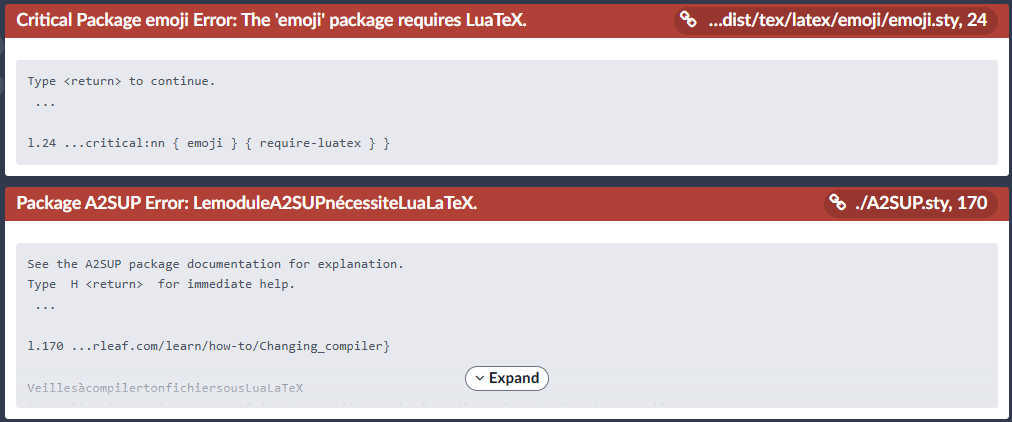
\includegraphics[width=0.8\linewidth]{img/erreur_lualatex.png}
\end{center}

\subsection{Compilation impossible}

Overleaf peut afficher ce message d'erreur :

\begin{center}
    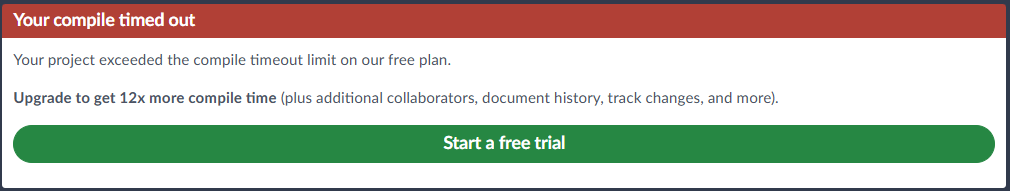
\includegraphics[width=0.8\linewidth]{img/compil_out.png}
\end{center}

Cela est dû aux restrictions du service gratuit d'Overleaf... Mais il existe deux alternatives à cela : Visual Studio Code (section \ref{VSC}) ; PLMLatex (section \ref{plmlatex}). 

\subsubsection{Visual Studio Code}\label{VSC}

Uniquement pour ceux possédant un ordinateur, il est possible d'installer le logiciel Visual Studio Code (en suivant le tutoriel ici : \url{https://shorturl.at/l8kYR}). Il utilisera alors les performances de l'ordinateur, largement suffisantes pour compiler n'importe quel support.\\

Néanmoins, je valorise la deuxième alternative, car plus rapide.

\subsubsection{PLMLatex}\label{plmlatex}

PLMLatex\footnote{\url{https://plmlatex.math.cnrs.fr}} est un site réalisé et entretenu par des mathématiciens français, ayant la volonté de mettre à disposition un site ayant à peu près les mêmes avantages qu'Overleaf, à tous les Français d'universités et institutions. Ainsi, vous avez à l'heure actuelle, un compte PLMLatex, via vos adresses universitaires @etu.u-paris.fr \emoji{smile}.\\

Le gros avantage que nous exploiterons, est la possibilité de compiler \textbf{n'importe quel} support, sans limitation de temps\footnote{En réalité, il est fixé à 10 min, mais le support doit être déraisonnablement long. Atteindre 10 min signifie surtout que nous rédigeons une thèse, ou un support dans lequel il y a une boucle infinie.}. Il présente donc l'avantage de Visual Studio Code, sans le côté lourd de l'installation/configuration ! Et pas des moindres, il est utilisable sur tablette et téléphone ! Il est donc en théorie possible de réaliser un tuto de A à Z sur téléphone \emoji{wink}.\\

Attention cependant, PLMLatex ne doit pas être utilisé pour travailler sur un projet. La collaboration pour les rédactions et relectures doit se faire au maximum sur Overleaf, pour éviter de multiplier des versions d'un même support. Idéalement, une fois qu'un projet a été compilé avec PLMLatex, il faudrait donc supprimer le projet \textbf{sur PLMLatex}, afin de ne conserver que la version originale Overleaf.



\subsection{\textsl{Missing a \$}}

\begin{center}
    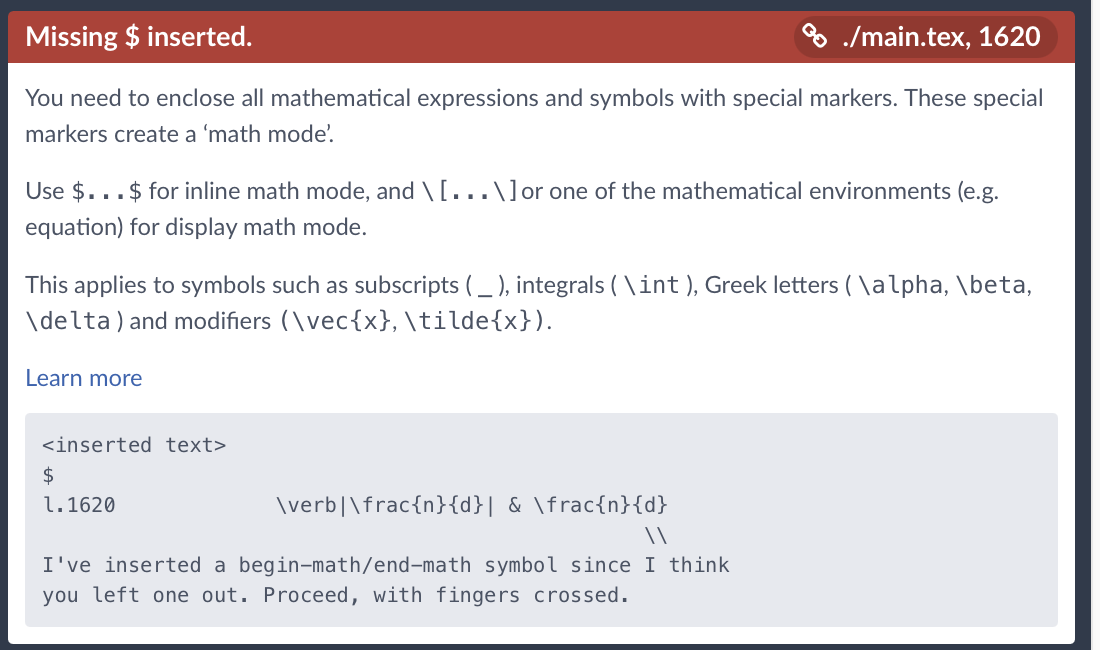
\includegraphics[width=0.7\linewidth]{img/no-dollar.png}
\end{center}

Cela signifie que vous avez dû ouvrir un mode \textsl{inline} ou \textsl{math}, et que vous avez oublié de le fermer, avec un \$. Concentrez-vous sur les passages où se trouvent des calculs, où des symboles tels que des lettres grecques, qui doivent être entourées de \$.


\subsection{LaTeX Error: The key ... is unknown and is being ignored}\label{key-error}

\begin{center}
    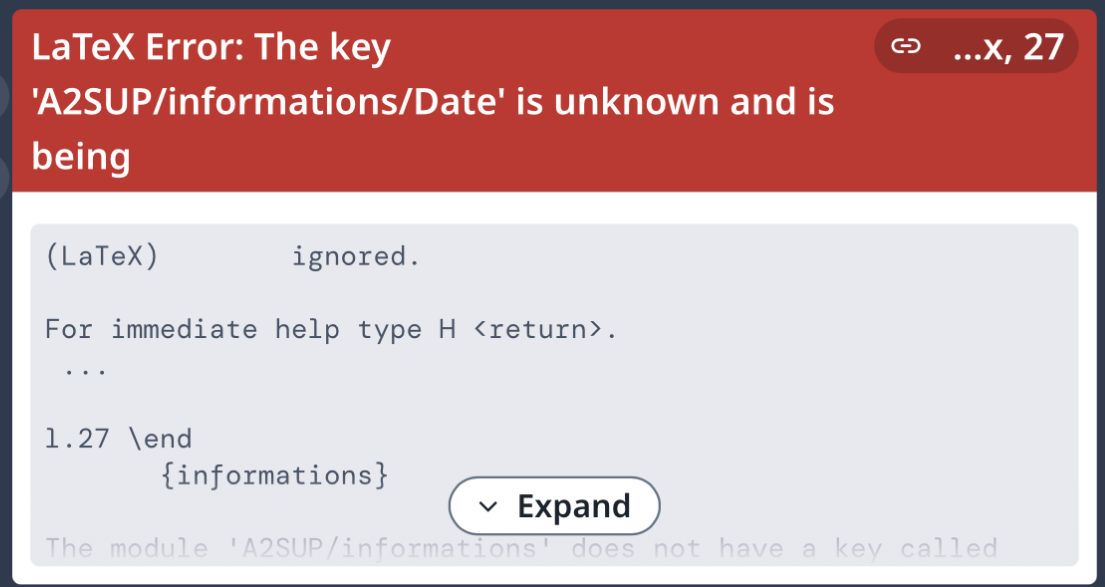
\includegraphics[width=0.7\linewidth]{img/key-error.png}
\end{center}

Cette erreur vient du fait qu'une ou plusieurs clés que vous avez indiquées dans l'environnement \verb|informations| n'existent pas en réalité. Si la ou les clés étaient utilisées auparavant, vérifiez qu'elles n'ont pas été retirées du package par la suite (exemple de la clé \verb|NombreDeQuestions|, qui n'existe plus, \LaTeX{} détectant automatiquement le nombre total de questions dans un support comme un tuto, ou encore la clé \verb|Date|, qui a été remplacée par \verb|Session| pour les annales).








\newpage
\section{Packages pré-importés par \texttt{A2SUP.sty}}

Pour bien fonctionner, le package \verb|A2SUP.sty| importe lui-même des packages. Voici les packages concernés :

\begin{itemize}
    \item amssymb
    \item babel
    \item bclogo
    \item chemfig
    \item dashrule
    \item emoji
    \item enumitem
    \item expl3
    \item fancyhdr
    \item geometry
    \item graphicx
    \item hyperref
    \item icomma
    \item l3draw
    \item lipsum
    \item lmodern
    \item chemmacros
    \item mdframed
    \item mhchem
    \item moresize
    \item pdfpages
    \item pifont
    \item pgfplots
    \item fillbetween
    \item pst-tree
    \item setspace
    \item tabularx
    \item varwidth
    \item tcolorbox
    \item tikz
    \item tkz-tab
    \item truncate
    \item realhats
    \item ulem
    \item wrapfig
    \item xcolor
    \item xstring
    \item titlesec
    \item scrextend
\end{itemize}

Si un package est manquant, ne pas hésiter à le proposer !



\newpage
\section{Support et retour}
Pour signaler des problèmes ou demander de nouvelles fonctionnalités, rendez-vous sur le salon \LaTeX{} du Discord A2SUP, ou contactez Abdussamed directement sur Discord (abdussamed.yzc) (ou Messenger, Abdussamed Yazici).


\newpage
% Annexe
\appendix
\section{Template} \label{template}

\begin{lstlisting}
\documentclass[12pt]{article}

\usepackage[...]{A2SUP}

\begin{informations}
    UE = ,
    Support = ,
    NumeroDuSupport = ,
    SujetOuCorrection = ,
    Orientation = ,
    Pagination = ,
    TiersTemps = ,
    RecoSpecifiques = ,
    TitreExtra = ,
    SousTitre = ,
    Redacteurs = {},
    Relecteurs = {},
    ConvertisseursLatex = {},
    Testeurs = {},
    TuteursEnSeance = {},
    VP = {},
    Team = ,
    RM = {},
    FacRedactionOuCollab = ,
    RemerciementsBonus = ,
    Session = ,
    RelectureProfs = ,
\end{informations}

\begin{document}
    \recto
    \grille
    \motRM

    \question{1}
    {Énoncé}
    {Item A}
    {Item B}
    {Item C}
    {Item D}
    {Item E}
    {AE}

    \begin{correction}
        \correctionitem{Items A et B}
        ...

        \correctionitem{Items C et D}
        ...
        
        \correctionitem{Item E}
        ...
    \end{correction}

    \verso
\end{document}
\end{lstlisting}

\section{Liste des commandes et environnements du package \texttt{A2SUP.sty}}

\begin{itemize}
    \item Commandes définies :
        \begin{itemize}[label=$\bullet$, font=\footnotesize]
            \item \verb|\recto|
            \item \verb|\grille|
            \item \verb|\question|
            \item \verb|\questionouverte|
            \item \verb|\correctionitem|
            \item \verb|\verso|
            \item \verb|\annexe|
            \item \verb|\pagevide|
            \item \verb|\reponse|
            \item \verb|\inseparable|
            \item \verb|\figanalyse|
            \item \verb|\brouillon|
        \end{itemize}
    \item Environnements :
    \begin{itemize}[label=$\bullet$, font=\footnotesize]
        \item \verb|informations|
        \item \verb|motRM|
        \item \verb|boite|
        \item \verb|inclure|
        \item \verb|memoire|
        \item \verb|correction|
        \item \verb|analyse|
    \end{itemize}
\end{itemize}




\section{Changelog}

\textbf{Version 2.0.3.2 (mercredi 20 août 23h34) :}

\begin{itemize}
    \item Ajout du logo discord au verso
\end{itemize}

\textbf{Version 2.0.3.1 (dimanche 17 août) :}

Par Semih YAZICI :

\begin{itemize}
    \item Réactualisation des visuels des supports de PASS
    \item Modification du verso PASS
    \item En attente des visuels de L.AS
\end{itemize}

\textbf{Version 2.0.2.1.4 (jeudi 02 décembre 03h37) :}

\begin{itemize}
    \item \verb|\inseparable| pouvait créer des décalages absurdes de texte sur le PDF. Ajout de \verb|\par| en fin d'environnement \texttt{correction} pour résoudre ce problème.
\end{itemize}


\textbf{Version 2.0.2.1.3 (mardi 31 décembre 23h40) :}

\begin{itemize}
    \item Ajout d'une version étoilée de la commande \verb|\correctionitem|, permettant d'empêcher le rappel d'item.
\end{itemize}

\textbf{Version 2.0.2.1.2 (lundi 30 décembre 14h19) :}

\begin{itemize}
    \item Modification de la valeur protégeant le bloc de correction (\verb|\needspace{\baseline*3}| plutôt que \verb|\needspace{\baseline*5}|).
\end{itemize}

\textbf{Version 2.0.2.1 (jeudi 26 décembre 13h53) :}

\begin{itemize}
    \item Petite modification pour rectifier l'information concernant l'autorisation des calculatrices selon les (EC)UE. Testé et confirmé.
\end{itemize}

\textbf{Version 2.0.2 (mercredi 25 décembre 23h08) :}

\begin{itemize}
    \item Ajout de l'environnement \texttt{analyse}, et des commandes associées \verb|\figanalyse| et \verb|\brouillon|.
\end{itemize}



\textbf{Version 2.0.1 (mercredi 25 décembre 01h57) :}

\begin{itemize}
    \item Légère modification, concernant la page de couverture des annales et tutos, prenant en compte l'existence ou non d'une page de remerciements pour le calcul du nombre total de pages dans le support.
\end{itemize}

\textbf{Version 2.0 (mardi 24 décembre 19h00) :}

\begin{itemize}
    \item Complément de description de la commande \verb|\recto|, à propos de l'argument optionnel et de la gestion des packs de fiches pour les L.AS
    \item Les deux versions \texttt{Archive PASS} et \texttt{Archive L.AS} sont maintenant fusionnées. L'unique projet \texttt{A2Latex} assurera maintenant la rédaction des supports pour les deux voies d'accès !
    \item La calculatrice autorisée a été prise en compte pour la Biophysique L.AS
    \item Changement des codes permettant de remplir la grille. Le code précédent, bien que fonctionnel, était long à exécuter (la compilation était donc relativement longue). Le nouveau code est donc plus optimisé.
\end{itemize}

\textbf{Version 1.2.1 (lundi 16 décembre 23h37) :}

\begin{itemize}
    \item Rectification de la commande \verb|\question|. La forme étoilée présentait un bug.
\end{itemize}

\textbf{Version 1.2 (dimanche 15 décembre 04h38) :}

\begin{itemize}
    \item La grille a été reprise, de façon à ce que \LaTeX{} la remplisse en accord avec les questions. Auparavant, la grille se remplissait au fur et à mesure, sans considérer les numéros de questions. À présent, la grille ira chercher la correspondance entre les bilans de réponses et les questions pour remplir les bonnes cases, ce qui peut être utile pour un support ne contenant pas toutes les questions (par exemple, question 1, puis question 3, la question 2 ayant donc été omise).
    \item La commande \verb|\question| a été modifiée : 
        \begin{itemize}
            \item elle a acquis une version étoilée, indiquant que la question est hors programme
            \item elle n'a plus d'argument optionnel consacré aux aides aux calculs. Il est plus pertinent d'intégrer les aides aux calculs dans le 2ème argument obligatoire de la commande, contenant l'énoncé (voir exemple de la section \ref{aide_au_calcul})
        \end{itemize}
\end{itemize}


\textbf{Version 1.1 (mercredi 11 décembre 01h53) :}

\begin{itemize}
    \item L'environnement \verb|informations| contient désormais une nouvelle clé : \verb|RelectureProfs|, qui prend pour valeur "oui", ou "non" ("non" par défaut). Elle permet, pour une correction, de ne pas afficher les corrections détaillées. Ainsi, les items seront mis en page selon les bilans de réponse. Il sera alors possible de transmettre le document aux professeurs, qui ne souhaitent généralement pas avoir accès à nos corrections détaillées.
    \item La documentation est plus précise concernant la commande \verb|\inseparable|
    \item La documentation recense une erreur commune en plus (voir section \ref{key-error})
\end{itemize}


\textbf{Version 1.0 (dimanche 8 décembre 00h57) :}

\begin{itemize}
    \item \verb|NombreDeQuestions| a été retiré. Il n'est plus nécessaire d'indiquer manuellement le nombre de questions total (ce dernier étant affiché en recto de tutos et annales).
    \item La grille a été entièrement recodée. Elle contenait des commandes compilables uniquement avec TexLive 2024 (PLMLatex et Visual Studio Code TexLive <2024 ne pouvaient donc pas compiler les projets).
    \item La définition des arguments obligatoires de la commande \verb|\question| a été changée, ce qui permet de mieux encoder les contenus complexes comme les environnements (du détail... mais si vous avez un problème avec la commande question, demandez-vous si vous avez la dernière version !).
    \item \verb|\questionouverte| a été légèrement modifiée de façon à ce que l'environnement \verb|correction| prenne bien en compte les questions ouvertes.
\end{itemize}

\textbf{Version 0.0 (avant le dimanche 8 décembre) :} Première version arbitraire.

\end{document}
